\PassOptionsToPackage{square,comma,numbers,sort&compress}{natbib}
\documentclass{article}

% if you need to pass options to natbib, use, e.g.:
%     \PassOptionsToPackage{numbers, compress}{natbib}
% before loading neurips_2021

% ready for submission
\usepackage[final]{neurips_2021}

% to compile a preprint version, e.g., for submission to arXiv, add add the
% [preprint] option:
%     \usepackage[preprint]{neurips_2021}

% to compile a camera-ready version, add the [final] option, e.g.:
%     \usepackage[final]{neurips_2021}

% to avoid loading the natbib package, add option nonatbib:
%    \usepackage[nonatbib]{neurips_2021}

\usepackage[utf8]{inputenc} % allow utf-8 input
\usepackage[T1]{fontenc}    % use 8-bit T1 fonts
\usepackage{url}            % simple URL typesetting
\usepackage{natbib} % has a nice set of citation styles and commands
\usepackage{booktabs}       % professional-quality tables
\usepackage{amsfonts}       % blackboard math symbols
\usepackage{nicefrac}       % compact symbols for 1/2, etc.
\usepackage{microtype}      % microtypography
\usepackage{xcolor}         % colors
\usepackage[frozencache,cachedir=.]{minted}
\usepackage[ruled,vlined,shortend, linesnumbered]{algorithm2e} % algorithm
\usepackage[]{algorithmic} % algorithm
\usepackage{tikz,tikzpeople}
\usepackage{amsmath}
\usepackage{todonotes}
\usepackage{wrapfig}
\usetikzlibrary{shapes.geometric}
\usepackage{graphicx}
\usepackage[inline]{enumitem}
\usepackage{pgfplots}
\pgfplotsset{compat=1.5}
\usepgfplotslibrary{groupplots}

\usepackage[hidelinks]{hyperref}       % hyperlinks
\definecolor{purple}{rgb}{0.7,0,1.0}
\newcommand{\mks}[1]{[\textcolor{purple}{$^{MK}_S$ \small #1}]}

\newcommand{\SpA}{{\textsc{SpliceOut}}\xspace}

\title{\SpA: A Simple and Efficient Audio Augmentation Method}

% The \author macro works with any number of authors. There are two commands
% used to separate the names and addresses of multiple authors: \And and \AND.
%
% Using \And between authors leaves it to LaTeX to determine where to break the
% lines. Using \AND forces a line break at that point. So, if LaTeX puts 3 of 4
% authors names on the first line, and the last on the second line, try using
% \AND instead of \And before the third author name.
% \setcounter{table}{10}
\author{%
  Arjit Jain \\
  Indian Institute of Technology Bombay\\
  \texttt{arjit@cse.iitb.ac.in} \\
  % examples of more authors
   \And
   Pranay Reddy Samala \\
   Indian Institute of Technology Bombay\ \\
   \texttt{pranayr@cse.iitb.ac.in} \\
   \AND
   Deepak Mittal \\
   Verisk Analytics \\
   \texttt{deepak.mittal@verisk.com} \\
   \And
   Preethi Jyothi \\
   Indian Institute of Technology Bombay\ \\
   \texttt{pjyothi@cse.iitb.ac.in} \\
   \And
   Maneesh Singh \\
   Verisk Analytics \\
   \texttt{maneesh.singh@verisk.com} \\
}

\begin{document}
% \iffalse
\maketitle

\begin{abstract}
Time masking has become a \textit{de facto} augmentation technique for speech and audio tasks, including automatic speech recognition (ASR) and audio classification, most notably as a part of SpecAugment. %However, time masking alters the statistics of the underlying data distribution which can inadvertently affect the network training. 
%In this work, we propose, \SpA, a simple modification to time masking which, in expectation, is consistent with the data distribution. 
In this work, we propose \SpA, a simple modification to time masking which makes it computationally more  efficient. \SpA performs comparably to (and sometimes outperforms) SpecAugment on a wide variety of speech and audio tasks, including ASR for seven different languages using varying amounts of training data, as well as on speech translation, sound and music classification, thus establishing itself as a broadly applicable audio augmentation method. \SpA also provides additional gains when used in conjunction with other augmentation techniques. Apart from the fully-supervised setting, we also demonstrate that \SpA can complement unsupervised representation learning with performance gains in the semi-supervised and self-supervised settings. %Finally, we motivate why \SpA might be a perceptually meaningful alternative to time masking. 
%By design, SnipAugment, is more compute, memory and time efficient than time masking. We show SnipAugment can serve as a direct replacement for Time Masking, and outperform Time Masking on a variety of different tasks, for both raw waveform based and spectrogram based input formats. Moreover, we show that SnipAugment can provide gains even when used in conjunction with Time Masking. Finally, we show how SnipAugment can complement Representation learning, and show improvements in Semi-Supervised and Self-Supervised setups. 
\looseness=-1
\end{abstract}

\section{Introduction}
Data augmentation has become an integral part of the modern machine learning pipeline. It involves applying label-preserving transformations to training data that increases diversity in the training samples, thus acting as a regularizer to prevent overfitting. Data augmentation has also emerged as an important technique in recent self-supervised and semi-supervised learning algorithms to help learn useful representations of the data~\citep{xie2020selftraining,grill2020bootstrap,chen2020exploring,zbontar2021barlow,caron2020unsupervised,he2020momentum,chen2020simple}. Augmentation techniques demonstrated a lot of initial success in image classification tasks~\citep{perez2017effectiveness} and have been adopted for text, speech and audio tasks as well~\citep{wei-zou-2019-eda,kobayashi-2018-contextual,hou-etal-2018-sequence}. For speech and audio-based applications, augmentations like vocal tract length transformations~\citep{jaitly2013vocal}, speed perturbations~\citep{speedpertubation} and adding environment noise were early techniques that were found to be effective. However, these techniques typically incur additional computational costs and sometimes require additional data (e.g. in noise-based augmentations).
\looseness=-1

SpecAugment~\citep{specaugment} offered a simple alternative of directly transforming an audio spectrogram (i.e. a visual representation of the audio signal) by randomly warping across the time axis or masking consecutive chunks of time (i.e. \emph{time masking}) or frequency channels (i.e. \emph{frequency masking}) in the spectrogram. It was shown to be very effective for ASR, and has since been used for audio classification tasks as well~\citep{panns,urban,deepspectrumlite}. Investigations into new augmentation techniques that work broadly across different audio and speech tasks have been fairly limited. This could be partly attributed to the opaque nature of the audio spectrogram. Unlike image transformations (e.g., translation, shear, brightness, etc.) or text transformations (e.g., synonym replacements, word swapping, etc.) whose effects on a training instance can be easily visualized and understood, transformations on audio spectrograms are harder to interpret, and thus more challenging to define.
\looseness=-1

In this work, we propose \SpA, a simple modification to time masking that makes it more computationally efficient. Instead of masking splices of consecutive time-steps in the audio input, \SpA operates by entirely removing these time slices from the audio input and stitching the remaining parts together. Figure~\ref{fig:spliceout} illustrates the main difference between \SpA and time masking. 
\looseness=-1

\begin{figure}[t!]
    \centering
    \includegraphics[width=\textwidth]{images/diagram.pdf}
    \caption{Illustration of \SpA and time masking.} 
    \label{fig:spliceout}
\end{figure}

%Drawing inspiration from prior work in auditory perception, we also motivate why \SpA might be a perceptually meaningful alternative to time masking.

%We demonstrate the utility of \SpA using a wide range of tasks including ASR, speech translation, audio and music classification. 
While augmentation techniques in prior work have been typically proposed for specific target tasks (e.g. SpecAugment for ASR), we present \SpA as a broadly applicable augmentation technique for most sequence labeling or multi-class classification tasks using speech or audio as input. We substantiate the claim that \SpA has broad applicability by showing that it performs as well as (and at times better than) time masking on many speech and audio tasks including ASR, speech translation, sound and music classification. (\SpA can be applied to both raw waveform and spectrogram-based input formats.) 
We demonstrate the effectiveness of \SpA in both low and high resource training regimes and show ASR results for a number of different languages. Besides fully supervised tasks, we also demonstrate that \SpA can benefit representation learning by showing improvements in semi-supervised and self-supervised settings. Along with establishing that \SpA is useful as a standalone technique, we also show that \SpA can be complementary to time masking. It is noteworthy that in all our experiments \SpA was used as a drop-in replacement for SpecAugment whose hyperparameters were presumably tuned for the task at hand; any performance improvements we derived with \SpA were  without using any separate hyperparameter tuning. 
%and it is effective when used in frameworks that learn policies for data augmentation.

%Data Augmentation is an important aspect of training modern machine learning systems. It has been shown to increase the diversity in training data in low resource setups, and act as a regularizer in supervised learning to prevent overfitting. Recent semi-supervised and self-supervised learning algorithms heavily rely on data augmentation methods for learning useful representations~\citep{xie2020selftraining,grill2020bootstrap,chen2020exploring,zbontar2021barlow,caron2020unsupervised,he2020momentum,chen2020simple}. 

%For example, in Computer Vision, image transformations are often used for data augmentation to encourage the network's output to be invariant to the given transformation. Representations that are invariant to common semantic-preserving image transformations have been shown to achieve better performance and generalization on downstream tasks~\citep{Misra_2020_CVPR}. However, defining such invariants for audio data is challenging, and tends to be highly task-specific. 
% For Automatic Speech Recognition (ASR), SpecAugment and Speed Pertubation, for Far-Field ASR, multi-channel noisy and reverberant speech with room simulators, Pitch Shifting for chord recognition, spectral filtering for music detection, mixup for environmental sound classification, and synthetic mixing for source separation. 
%The idea being that different tasks require very different augmentations. 
%The different representations of the input, waveform and spectrogram-based, further adds up to the challenge. 

%As a result, much of the recent research has been on investigating end-to-end network architectures specialized for different tasks, e.g. automatic speech recognition (ASR), and works discussing audio augmentations and transformations are fairly limited. Time Masking is one of the few techniques that is applicable, and shown to be effective in a wide range of speech and audio tasks. The most widely adopted implementation of time masking is to mask continuous intervals of time-steps, and thus, it is compatible with both waveform and spectrogram-based representations. The latter is part of SpecAugment~\citep{specaugment}, the de facto data augmentation strategy for speech data. 

%In this work, we propose \SpA, a simple modification to time masking which makes it more computationally efficient. We show that \SpA outputs samples that are consistent with the input data with respect to summary statistics~\citep{summary1}, and motivate why \SpA might be a perceptually meaningful alternative to time masking.

%\SpA performs at least at par, often improving upon, time masking on a variety of speech and audio tasks spanning different model architectures, when applied to both raw waveform and spectrogram-based input formats. Moreover, we show that \SpA is complementary to time masking, and SpecAugment. We demonstrate the effectiveness of \SpA in the low-resource regime, and on multilingual datasets. Apart from fully-supervised settings, we also demonstrate that \SpA can complement representation learning by showing improvements in semi-supervised and self-supervised settings. 

\section{Related Work}

Masking-based augmentation (and regularization) techniques have been used extensively in machine learning, from masking weights~\citep{germain2015made} and hidden states~\citep{dropout,autodropout,ghiasi2018dropblock,pmlr-v28-wan13} in neural networks, to masking pixels in images~\citep{devries2017improved,Zhong_Zheng_Kang_Li_Yang_2020,8100170,10.1145/344779.344972}, words in text~\citep{devlin2018bert,donahue-etal-2020-enabling,gal2016theoretically}, and time-steps in audio~\citep{specaugment,clar} and time-series data. While masking has been employed as a commonly used augmentation technique, it has also been used in representation learning where the objective involves learning to reconstruct masked out information~\citep{donahue-etal-2020-enabling,10.1145/344779.344972,devlin2018bert}; this reconstruction objective forms the basis of most of the recent semi-supervised and self-supervised learning approaches. Masking-based augmentation techniques can also be used with contrastive losses for representation learning (that have seen a recent resurgence~\citep{zbontar2021barlow,chen2020simple,he2020momentum} where different augmented views of the same data samples can serve as positive examples.

\paragraph*{Audio Augmentations.} Audio augmentation techniques can be broadly classified into the following categories: \begin{enumerate*}
\item \textbf{Warping-based:} Changing the speed of the audio signal using time warping techniques was shown to be effective as an augmentation for ASR~\citep{speedpertubation}.
Both time warping~\citep{specaugment} and frequency warping~\citep{jaitly2013vocal} have been used to augment training examples for ASR.
%SpecAugment~\citep{specaugment} also employs time warping along random points on the time axis as an augmentation policy for ASR. Frequency warping (c.f., vocal tract length normalization techniques~\citep{vtln} used for speaker normalization) has also been used to augment training examples for ASR~\citep{jaitly2013vocal}.
\item \textbf{Mixing-based:} Mixup~\citep{zhang2018mixup} involves creating new training samples using linear combinations of existing data samples (and their corresponding labels). Mixup was shown to be very effective for audio classification~\citep{panns} and it has also been used successfully for ASR~\citep{mixupasr,meng2021mixspeech}. Related to mixing, reordering shuffled patches of a spectrogram or swapping parts of a spectrogram have also been explored for audio augmentation ~\citep{Carr_2021,specswap}.
\item \textbf{Masking-based:} Time masking and frequency masking~\citep{specaugment} are the most popular audio masking techniques that work by zeroing out randomly chosen blocks of consecutive time steps and frequency channels, respectively. CutMix~\citep{yun2019cutmix} is a recent augmentation technique combining mixing and masking that has been shown to work well for audio classification~\citep{deepspectrumlite}.
\item \textbf{Noise-based:} Augmenting training data with synthesized noisy speech samples~\citep{deepspeech} and simulated reverberant conditions~\citep{ko2017study,kim2017generation} was found to improve ASR on noisy speech and far-field ASR.
\end{enumerate*} 

In addition to the above-mentioned methods, augmentation techniques specific to a target task, such as using text-to-speech synthesis for ASR~\citep{tjandra2017listening,karita2019semi,wang2020improving}, extending masking and mixing to hidden states for audio classification~\citep{specaugmentpp} have also demonstrated benefits.

\SpA shares similarities with frame skipping/dropping methods~\cite{dynamicframeskipping,45555,7472084,6639137} in that both offer computational advantages by ignoring parts of the input. We compare \SpA with these methods in Appendix \ref{app:frameskipping}

\SpA would qualify as a time masking technique, except we delete blocks of consecutive time-steps instead of masking them. In subsequent experimental comparisons, we use \SpA as a drop-in replacement for time masking. \SpA is also complementary to other augmentation techniques as will be demonstrated in Section~\ref{sec:expts}. 

%{In addition to the above methods, several new paradigms and extensions have also been proposed recently. For instance, Masking and Mixing based augmentations have been extended to hidden states~\citep{specaugmentpp}. Other augmentation methods include using Voice Conversion and Text-To-Speech models, Phase Shuffle~\citep{donahue2019adversarial}, Pitch and Time Shift, Reverberation, Dynamic Range Compression, MP3Compression and Fade In/Out~\citep{librosa,clar}. Also, contextualize \SpA with prior work.}

\iffalse
Masking based techniques have been used extensively in machine learning, from masking weights~\citep{germain2015made}, and hidden states~\citep{dropout,autodropout,ghiasi2018dropblock,pmlr-v28-wan13} in neural networks, to masking pixels in images~\citep{devries2017improved,Zhong_Zheng_Kang_Li_Yang_2020,8100170,10.1145/344779.344972}, words in text~\citep{devlin2018bert,donahue-etal-2020-enabling,gal2016theoretically}, and time steps in audio~\citep{specaugment,clar}. The usage of masking can be broadly classified into two categories depending on how the masked out information is incorporated in the learning objective: implicit prediction, and explicit prediction. The former includes cases where masking is used as a data transformation or augmentation technique, and the latter involves learning to reconstruct the masked out information~\citep{donahue-etal-2020-enabling,10.1145/344779.344972,devlin2018bert}, forms the basis of most of the recent semi-supervised and self-supervised learning approaches. 

\subsection{Audio Augmentations}
Our work relates to transformations and augmentations on audio data, broadly classified as 

\textbf{Mixing based} Mixup~\citep{zhang2018mixup} involves taking linear combination of data samples, and their corresponding labels, to create new examples for training and is extremely effective in Audio Classification~\citep{panns}, with recent extensions to ASR~\citep{meng2021mixspeech}. Intra-Sample mixing and permutation have also been tried in~\citep{Carr_2021,specswap}

\textbf{Masking based}
The two major methods, Time Masking and Frequency Masking  zero out the time steps, and frequency channels respectively, in a randomly selected interval~\citep{specaugment}. CutMix~\citep{yun2019cutmix}, a combination of Mixing and Masking,  has also been used for audio classification~\citep{deepspectrumlite}.
% Time Masking and Frequency Masking zero out the time steps, and frequency channels respectively, in a randomly selected interval~\citep{specaugment}. CutMix~\citep{yun2019cutmix} has also been used for audio classification~\citep{deepspectrumlite}.

\textbf{Speed based} 
Speed Pertubation~\citep{speedpertubation} changes the speed of the audio signal, Time Stretch and Time Warping~\citep{specaugment} involve streching and squeezing time windows in raw waveforms and spectrograms respectively. 

\textbf{Noise based} Methods involves adding random white, brown or pink noise. Gaussian noise based modification, depending on the Signal to Noise Ratio, are also common.

In addition to the above methods, several new paradigms and extensions have also been proposed recently. For instance, Masking and Mixing based augmentations have been extended to hidden states~\citep{specaugmentpp}. Other augmentation methods include using Voice Conversion and Text-To-Speech models, Phase Shuffle~\citep{donahue2019adversarial}, Pitch and Time Shift, Reverberation, Dynamic Range Compression, MP3Compression and Fade In/Out~\citep{librosa,clar}. 

Give some explanation for why we are only comparing with time masking: Most of these methods are complementary to SpecAug. So they should be directly compatible with \SpA
\fi

\section{\SpA}
%\subsection{Method}
\SpA is parameterized by $N$, the number of time intervals to splice, and $T$, the maximum width of a time interval. Given a log-mel spectrogram with $\tau$ time steps, \SpA selects $N$ intervals, each of the form $[t_0, t_0+t)$ where $t \in \mathbb{Z}^{0+}$ is sampled from the uniform distribution $U(0, T)$, and $t_0 \in \mathbb{Z}^{0+}$ is chosen from $[0, \tau - t)$. The input spectrogram is modified by removing all time steps in the union of the selected intervals. NumPy-style pseudocode for both \SpA and Time-masking is outlined below in Algorithms~\ref{alg:spliceout} and~\ref{alg:tm}. 

\begin{minipage}{0.46\linewidth}
\begin{algorithm}[H]
\caption{Pseudocode for \SpA}
\label{alg:spliceout}
\begin{minted}{python}
def SpliceOut(spec, N, T):
  tau = spec.shape[0]
  mask = np.ones(tau, dtype=bool)
  for i in range(N):
    length = randint(T)
    start = randint(tau-length)
    mask[start:start+length] = False
  spec = spec[mask]
  return spec
\end{minted}
\end{algorithm}
\end{minipage}
\hfill
\begin{minipage}{0.46\linewidth}
\begin{algorithm}[H]
\caption{Pseudocode for Time-Masking}
\label{alg:tm}
\begin{minted}{python}
def TimeMasking(spec, N, T):
  tau = spec.shape[0]
  for i in range(N):
    length = randint(T)
    start = randint(tau-length)
    spec[start:start+length] = 0
  return spec
\end{minted}
\end{algorithm}
\end{minipage}
\paragraph{Computational Efficiency.} 

Figure \ref{fig:spliceout} illustrates how \SpA decreases the length of the output spectrogram, as opposed to Time-Masking which results in an output spectrogram of the same length as the original input spectrogram. As we increase the amount of masking, \SpA deletes larger numbers of time intervals from the input data, and the resulting shorter inputs in turn reduce the memory footprint, and time, required for training. Time-Masking, on the other hand, does not gain any computational advantage with respect to the memory or the time required for training, with increased amount of masking.

%On the other hand, on varying the amount of masking, we expect Time Masking to remain indifferent with respect to the memory or time required for training.
%
\begin{figure}
\label{fig:maskimprovements}
\centering
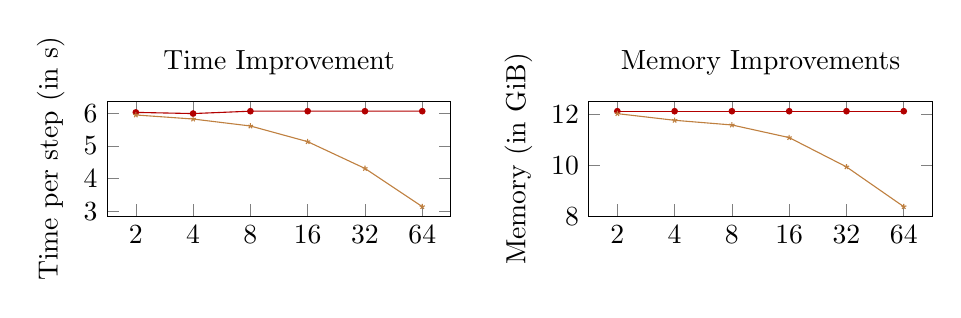
\begin{tikzpicture}
\pgfplotsset{
      scale only axis,
      width=0.3\textwidth,height=0.15\textwidth
  }

%   \begin{axis}[
%     axis y line*=left,
%     xlabel=Number of Masks,
%     xtick = {2, 4, 8, 16, 32, 64},
%     xmode = log,
%     log ticks with fixed point,
%     legend style={at={($(0,0)+(1.75cm,0.7cm)$)},legend columns=1,fill=none,draw=black,anchor=center,align=center},
%     tick label style={font=\normalsize},
%     ylabel = {Time per step (in s)},
%   ]
    
%     \addlegendentry{Time-Masking};    
%     \addlegendentry{\SpA};         

%     \end{axis}

%     \begin{axis}[
%       axis y line*=right,
%       axis x line=none,
%       xtick = {2, 4, 8, 16, 32, 64},
%       xmode = log,
%       log ticks with fixed point,
%         ytick = {8, 10, 12},
%         ymin==7.5,
%         ymax=12.5,
%         yticklabels = {$8$, $10$, $12$},
%         tick label style={font=\normalsize},
%         ylabel = {Memory (in GiB)},
%     ]

%   \end{axis}
\begin{groupplot}[group style={group size= 2 by 1,ylabels at=edge left, horizontal sep=1.75cm},width=0.36\textwidth,height=0.12\textwidth]
\nextgroupplot[label style={font=\normalsize},
xtick = {2, 4, 8, 16, 32, 64},
xmode = log,
log ticks with fixed point,
tick label style={font=\normalsize},
legend style={at={($(0,0)+(1cm,1cm)$)},legend columns=7,fill=none,draw=black,anchor=center,align=center},
ylabel = {Time per step (in s)},
legend to name=fredself1,
title = Time Improvement,
mark size=1pt]
\addplot[red!70!black,mark=*] coordinates {(2,6.024096386)
    (4,5.988023952)
    (8,6.060606061)
    (16,6.060606061)
    (32,6.060606061)
    (64,6.060606061)
    };
    \addplot[brown,mark=star] coordinates {(2,5.94530321)
    (4,5.820721769)
    (8,5.60758145)
    (16,5.128205128)
    (32,4.308487721)
    (64,3.138731952)
    };
\addlegendentry{Time-Masking};    
\addlegendentry{\SpA};
\coordinate (c1) at (rel axis cs:0,1);

\nextgroupplot[label style={font=\normalsize},
xtick = {2, 4, 8, 16, 32, 64},
xmode = log,
log ticks with fixed point,
tick label style={font=\normalsize},
ylabel = {Memory (in GiB)},
title = Memory Improvements,
mark size=1pt]
\addplot[red!70!black,mark=*] coordinates {(2,12.12207)
    (4,12.12207)
    (8,12.12207)
    (16,12.12207)
    (32,12.12207)
    (64,12.12207)
    };
    \addplot[brown,mark=star] coordinates {(2,12.026367)
    (4,11.764648)
    (8,11.581055)
    (16,11.084961)
    (32,9.9345703)
    (64,8.37207)
    };     
\end{groupplot}

\end{tikzpicture}
{\pgfplotslegendfromname{fredself1}};
% \includegraphics[width=0.5\textwidth]{images/eff.pdf}
\caption{Comparison of running time and memory requirements during training using Time-Masking and \SpA augmentations, with varying number of masks.}
\label{fig:efficiency}
%{The running time and memory required for training decrease as the number of masks is increased in \SpA, but remains constant for Time-Masking.}
\end{figure}

We empirically verify this for an ASR task on the LibriSpeech $100$-hr benchmark. (Details of the experimental setup and the model configuration are described in Section \ref{sec:libri}.) 
% We now isolate and compare only TM and \SpA augmentations with increasing the number of masks, $N$, while keeping the maximum width, $T$ constant. The task, datasets, and model configuration is the same as in Section \ref{sec:libri}. 
Figure \ref{fig:efficiency} plots the time taken per training step, and the memory required for training, for both Time-Masking and \SpA, for different values of $N$, while keeping the maximum width $T$ constant at $40$ time steps. As expected, we observe that \SpA is indeed more time-efficient and memory-efficient than Time-Masking. At an extreme level of masking i.e., $N=64$, \SpA achieves almost $2\text{x}$ speedup in training, and requires $33\%$ less memory. For a moderate masking level, $N=8$, \SpA achieves $8\%$ speedup in training, and requires $\sim 5\%$ less memory. For a fixed masking budget, we see that \SpA is more computationally efficient than Time-Masking, with larger gains as we increase the amount of masking. (ASR performance on Librispeech $100$-hr with varying number of masks is given in Section~\ref{sec:libri}.) 

\section{Experiments}
\label{sec:expts}

We demonstrate the effectiveness of \SpA on a wide variety of speech and audio tasks spanning different model architectures,  learning paradigms and toolkits. Table~\ref{tab:summary} summarizes the main tasks and datasets used in our experiments. We start with a well-known benchmark for English ASR, Librispeech~\citep{librispeech}. We present low-resource ASR results for many languages from the CommonVoice corpus~\citep{commonvoice} and show significant improvements in performance using \SpA. We also show performance improvements using \SpA on a speech translation task  Libri-Trans~\citep{libritrans}, translating English speech into French text. Apart from the sequence labeling tasks, we also evaluate \SpA using two popular sound classification tasks, ESC-50 and UrbanSound8K, and a music genre classification task. Finally, we show how \SpA helps learn better speech representations when trained using semi-supervised and self-supervised objectives. 

For significance analyses on ASR, we use Bootstrap Confidence Intervals (BCI)~\citep{bootstrap}, a widely adopted method for ASR performance evaluation, and for classification, we use the standard deviation obtained from cross-validation on predefined folds. Additional details about the significance and confidence analyses can be found in Appendix. 

%Additional details about the significance and confidence analyses can be found in Appendix A.1. 

%\todo[inline]{Things for the appendix.Implementation details for all experiments. Background on other works, like SimCLR, SapAugment, wav2vec2, conformer etc. Time taken for each experiment in the appendix. Evaluation metrics definitions. Dataset details (how many hrs and speakers and stuff). License of all codes and datasets that we used. IMP: Statistical significance of our experiments: K-Fold cross validation for Classification. Bootstrap Confidence intervals for Speech Recognition and Translation.} 

 Machine specifications and complete implementation details can be found in Appendix A.1. Appendix A.2 describes the datasets and frameworks we use, along with their respective licenses. Appendix A.3 explores the use of TM and \SpA with Sample Adaptive Policies~\citep{sapaugment} that help learn policies to automatically combine augmentation methods. Appendix A.4 shows how \SpA can be used to learn with noisy data, Appendix A.5 compares TM and \SpA as data augmentations to fine-tune a pre-trained wav2vec2 model using raw waveforms from TIMIT as input, and Appendix A.6 uses \SpA with raw waveforms for representation learning. Appendix A.7 supplements results from Table~\ref{tab:commonvoice} by extending to more languages from the CommonVoice corpus. 

\begin{table}
    \caption{A collated summary of the different tasks used to evaluate \SpA, along with the corresponding input representations, types of tasks, models and datasets.}
    \centering
    \begin{tabular}{llllll}
    \toprule
    Audio as & Task & Format & Type & Model & Datasets\\
    \midrule
    Speech & Recognition & Spectrogram & High Resource & Conformer & LibriSpeech-100\\
    &&&& Transformer & \\
    &&& Low Resource & Conformer & CommonVoice\\
    && Waveform & Fine-Tuning & Wav2Vec2 & TIMIT\\
    & Translation & Spectrogram & High Resource & & LibriTrans (En-Fr)\\
    & Classification & Spectrogram & Semi-Supervised & Resnet18 & SpeechCommands\\
    &&& Self-Supervised && \\
    && Waveform & Semi-Supervised & Resnet18 & \\
    &&& Self-Supervised &  & \\
    \midrule
    Sound & Classification & Spectrogram & Fine-Tuning & CNN10 & ESC-50, US8K\\
    &&& Self-Supervised & Resnet-18 & FSDNoisy18K\\
    &&& Pseudo-Labeling & DenseNet & \\
    \midrule
    Music & Classification & Spectrogram & Fine-Tuning & CNN14 & GTZAN \\
    \bottomrule
    \end{tabular}
    \label{tab:summary}
\end{table}

% \iffalse
% \begin{enumerate}[label=\textbf{\Alph*)},ref=\Alph*,leftmargin=*]
% \item \textbf{CommonVoice:} The CommonVoice corpus is a multilingual corpus of read speech in 38 languages. We train ASR models for nine different languages spanning training sets of varying sizes, ranging from 10 hours to 116 hours: Czech, Dutch, Kyrgyz, Russian, Swedish, Tatar, Turkish, Ukranian and Welsh. \todo{Mention how the train/dev/eval splits were chosen.}
% \item \textbf{Libri-Trans:} Libri-Trans is a spoken translation benchmark. It is an augmentation of Librispeech that contains approximately $240$h of English read speech aligned with French text. \todo{What's the train/dev/test split?}
% \item \textbf{ESC-50} and \textbf{Urban-Sound8K}: These are two well-known benchmarks for sound classification. \todo{More about how many class labels in each, train/dev/test splits.} 
% \item GTZAN: The GTZAN dataset is used for music genre classification. \todo{number of labels, train/dev/test splits}.
% \item Speech Commands$-10$ dataset: 
% \end{enumerate}
% \fi

\subsection{Speech-based Sequence Labeling Tasks}

\subsubsection{ASR: LibriSpeech}
\label{sec:libri}

Librispeech is a widely used ASR benchmark consisting of English read speech. We use the clean $100$-hr subset for training and evaluate on the standard dev (clean/other) and test (clean/other) sets. The ``other" evaluation datasets comprise speech samples that are more acoustically challenging. Our base model is the large variant of the Conformer model~\citep{conformer}, Conformer(L), which is a state-of-the-art network for ASR and is implemented using the ESPnet toolkit~\citep{espnet}. We use $83$-dimensional log mel-filterbank + pitch features as input. Each model is trained for $60$ epochs, and model averaging is performed on weights from $5$ epochs with the best performance on the validation set. Speed perturbation, with speeds $0.9, 1.0, 1.1$, is applied to the training data. Beam search is used during decoding, without invoking any external language model.
% More implementation details and hyperparameter values can be found in Appendix~\ref{sec:implementationdetails}.

%We compare \SpA with Time-Masking (TM), and it variants, with different combinations of Frequency Masking (FM), and Time-Warp (TW) on the widely benchmarked LibriSpeech 100hr dataset. $80$ dimensional log-mel filterbanks with $3$ dimensional pitch features are used for training. The base architecture is the large variant of the Conformer model, Conformer(L), a state-of-the-art network for ASR. Each model is trained for $60$ epochs, and model averaging is performed on weights from $5$ epochs with the best performance on the validation set. Mention Byte-Pair encoding. Speed Pertubation is applied to the training data, with speeds $0.9, 1.0, 1.1$. Beam search is used for decoding, without any external language model. 
%We use the espnet framework for conducting these experiments. All training related hyper-parameters were set to their default value, as used by espnet, and can be found in Appendix \ref{sec:implementationdetails}.  

\begin{table}
% \parbox{.40\linewidth}{    
\centering
    \caption{WERs on LibriSpeech test sets, using TM, FM and \SpA (SO), with $N=2$.}
    \begin{tabular}{lrr}
    \toprule
     Augmentation & test-clean & test-other\\
    \midrule
    % TM (Scale) & $9.7$ & $7.7{\scriptstyle \pm 0.19}$ & $25.8$ & $21.8{\scriptstyle \pm 0.31}$\\
    TM & $7.6{\scriptstyle \pm 0.19}$ & $21.8{\scriptstyle \pm 0.31}$\\
    SO & $\mathbf{7.5}{\scriptstyle \pm 0.18}$ & $\mathbf{21.4}{\scriptstyle \pm 0.31}$\\
    \midrule
    FM + TM & $\mathbf{7.2}{\scriptstyle \pm 0.17}$ & $18.3{\scriptstyle \pm 0.28}$\\
    FM + SO & $\mathbf{7.2}{\scriptstyle \pm 0.18}$ & $\mathbf{18.2}{\scriptstyle \pm 0.29}$\\
    \midrule
    % TW + FM + TM (Zero) & $7.1{\scriptstyle \pm 0.17}$ & $18.1{\scriptstyle \pm 0.29}$\\
    TW + FM + TM~\citep{specaugment,espnet} & $\mathbf{7.0}{\scriptstyle \pm 0.16}$ & $18.1{\scriptstyle \pm 0.28}$\\
    TW + FM + SO & $7.1{\scriptstyle \pm 0.17}$ & $17.9{\scriptstyle \pm 0.29}$\\
    TW + FM + TM + SO & $7.1{\scriptstyle \pm 0.18}$  & $\mathbf{17.7}{\scriptstyle \pm 0.29}$\\
    \bottomrule
    \end{tabular}
    \label{tab:libriaugs}
\end{table}


Table~\ref{tab:libriaugs} shows the word error rates (WERs) using \SpA as a replacement for Time-Masking (TM), both with and without the presence of other augmentations like time warping (TW) and frequency masking (FM). The time warp parameter for TW is set to $5$. We use $2$ masks of maximum width $30$ for FM. For TM and \SpA, $N=2$ and $T=40$. We observe that \SpA either performs comparably or a bit better when used as a replacement for TM. Interestingly, using \SpA in conjunction with SpecAugment (TW, FM, TM) yields further improvements in performance on test-other. Table \ref{tab:librimasks} shows how WERs change with increasing $N$ for TM and \SpA. For a fixed $N$, we observe that \SpA almost consistently outperforms TM. (With larger values of $N \ge 16$, the performance starts to degrade.)

%For Frequency Masking, the number of masks is set to $2$, and the max frequency width is set to $30$. For Time Masking, and it's variants, and \SpA, $N$ is set to $2$, and $T$ is set to $40$. 
%Table \ref{tab:libriaugs} compares TM and \SpA, when used in conjuction with TW, and FM. Write one line about TER and WER, and how lower is better. 
%We notice that \SpA achieves comparable performance with TM, and often outperforms TM. Interestingly, \SpA can be used along with SpecAugment (TW+FM+TM), and further improve performance on the test set. 
% \hfill
% \parbox{.45\linewidth}{
\begin{table}
    \centering
    \caption{Effect of increasing the number of masks, $N$, in Time-Masking and \SpA (SO) augmentations, on WERs of LibriSpeech test sets.}
    \begin{tabular}{rlrrrr}
    \toprule
    %  & & \multicolumn{2}{c}{Test Clean} & \multicolumn{2}{c}{Test Other}\\
    %  \cmidrule(r){3-6}
    N & Method & test-clean & test-other\\
    \midrule
    $2$ & TM & $7.6 {\scriptstyle \pm 0.19}$ & $21.8{\scriptstyle \pm 0.31}$\\
    & SO & $\mathbf{7.5}{\scriptstyle \pm 0.18}$ &  $\mathbf{21.4}{\scriptstyle \pm 0.31}$\\
    \midrule
    $4$ & TM  & $7.3{\scriptstyle \pm 0.18}$  & $20.4{\scriptstyle \pm 0.30}$\\
    & SO & $\mathbf{7.0}{\scriptstyle \pm 0.16}$ & $\mathbf{20.3}{\scriptstyle \pm 0.31}$\\
    \midrule
    $8$ & TM & $\mathbf{6.8}{\scriptstyle \pm 0.17}$  & $19.2{\scriptstyle \pm 0.29}$\\
    & SO  & $\mathbf{6.8}{\scriptstyle \pm 0.18}$ & $\mathbf{19.0}{\scriptstyle \pm 0.30}$\\
    \bottomrule
    \end{tabular}
    \label{tab:librimasks}
% }
\end{table}

\paragraph*{Semantic Mask.} While SpecAugment randomly masks time intervals in a spectrogram, Semantic-Mask~\citep{semanticmask} proposes masking out regions which correspond to a word or word-piece in the transcription, thus encouraging the decoder to learn a better internal language model. Similar to how we modify TM to implement \SpA, we modify Semantic-Mask to implement Semantic-Splice wherein we splice, or delete, certain intervals which correspond to a word or word-piece. We compare Semantic-Mask and Semantic-Splice on the LibriSpeech $100$-hr dataset. We follow the experimental setup described in ~\citep{semanticmask}, i.e. we use the Montreal Forced Aligner to compute forced alignments between the acoustic features and transcriptions. $15\%$ of the tokens are masked or spliced out in Semantic-Mask and Semantic-Splice, respectively. A transformer model is used as the base architecture, with convolutional layers for encoding, instead of positional encodings, similar to~\citep{semanticmask}. Speed pertubation, with speeds $0.9, 1.0, 1.1$ is used, along with SpecAugment. Models for both Semantic-Mask and Semantic-Splice were trained for $120$ epochs, and the model with the best validation performance was used for testing. Table \ref{tab:semantic} reports WERs for both methods showing that Semantic-Splice consistently outperforms Semantic-Mask on both the test sets. 

\begin{table}[h]
    \centering
    \caption{WERs on LibriSpeech test sets comparing Semantic-Mask and Semantic-Splice.}
    \begin{tabular}{lrr}
    \toprule
     Method & test-clean & test-other\\
    \midrule
    Semantic-Mask~\cite{semanticmask} & $9.2$ & $22$\\
    Semantic-Splice (Ours) & $\mathbf{8.8}$ & $\mathbf{21.5}$\\
    \bottomrule
    \end{tabular}
    \label{tab:semantic}
\end{table}

%reports the Test error rates with increasing number of masks for TM, and \SpA. We notice that both TM and \SpA provide gains on Test Error rates with increasing $N$. For a fixed $N$, \SpA slightly outperforms TM.


% Move this to the appendix. Right now, the settings and experiments are pretty confusing.
% \iffalse
% The CommonVoice corpus~\citep{commonvoice} is a multilingual corpus of read speech in 38 languages. We train ASR models for nine different languages spanning training sets of varying sizes, ranging from 10 hours to 116 hours: Czech, Dutch, Kyrgyz, Russian, Swedish, Tatar, Turkish, Ukranian and Welsh. We use a conformer architecture adapted for ESPnet\citep{espnetconformer} (more details are in Appendix A.1).
\subsubsection{ASR for Multiple Languages: CommonVoice}
\label{sec:commonvoice}
The CommonVoice corpus~\citep{commonvoice} is a multilingual corpus of read speech in 38 languages. We train ASR models for six different languages spanning training sizes ranging from 10 hours to 96 hours: Kyrgyz, Swedish, Tatar, Turkish, Ukranian and Welsh. We use a conformer architecture adapted for ESPnet\citep{espnetconformer} (more details are in Appendix A.1). The same model architecture and hyperparameter settings are used for all languages. We train the model for $50$ epochs with $83$-dimensional features ($80$ log-mel filterbank and $3$ pitch) and byte pair encoding (BPE)-based encoded transcripts (with a vocabulary of size 150. Speed perturbation is applied, with speeds $0.9$, $1.0$ and $1.1$, during training. Evaluation is done by averaging the $10$ models with the best validation accuracy. Beam search decoding without external language model is used during inference. Parameter values for TW, FM, TM are the same as in Section~\ref{sec:libri}.

%The parameters utilized for SpecAugment are maximum time warp $5$ for time warping, $2$ masks and $30$ maximum frequency width for frequency masking, and $2$ masks and $40$ maximum time width for time masking. For validation \SpA, we perform the same experiment replacing time masking, keeping all the parameters same. 
Table~\ref{tab:commonvoice} shows WERs for all six languages. Our experiments demonstrate that \SpA consistently outperforms TM, and  obtains statistically significant WER reductions on four low-resource languages, Kyrgyz, Swedish, Tatar and Ukrainian (at $p<0.05$ using the MAPSSWE test preferred for ASR evaluations~\citep{gillick1989some}). 
%As we observe from the results in Table \ref{tab:commonvoice}, \SpA consistently improves Word Error Rate, irrespective of the dataset size or language. 

\begin{table}[h!]
    \centering
    \caption{Evaluation of TM and \SpA, when used with TW and FM, using test WERs across multiple different languages, including several low-resource settings.}
    \begin{tabular}{l|rrrrr|r}
    \toprule
     Augmentation & Swedish  & Turkish  &  Kyrgyz & Ukrainian & Tatar & Welsh\\
    TW + FM & 10 hrs & 22 hrs & 22 hrs & 25 hrs & 28 hrs & 96 hrs\\ 
    %  Augmentation & Dev & Test & Dev & Test & Dev & Test & Dev & Test & Dev & Test\\
    \midrule
     + TM~\citep{specaugment,espnet} & $33.2$ &  $6.7$  & $37.3$ & $14.6$ & $36.3$ & $15.4$\\
     + \SpA & $\mathbf{32.1}$ & $\mathbf{6.5}$ & $\mathbf{36.2}$ & $\mathbf{14.0}$ & $\mathbf{35.5}$ & 
      $\mathbf{14.8}$\\
    % \midrule
    % & Model & Test & Model & Test & Model & Test & Model & Test & Model & Test \\
    % \midrule
    % SOTA & \citep{xlsr} & $25.31$ & \citep{wav2vec2} & $13.7$ & \citep{xlsr} & $14.3$ & \citep{xlsr} & $26.76$ & \citep{xlsr} & $31.88$\\
    \bottomrule
    \end{tabular}
    \label{tab:commonvoice}
\end{table}
\iffalse
\begin{table}[]
    \centering
    \caption{Additional CommonVoice languages}
    \begin{tabular}{lrrrrrrrrrr}
    \toprule
     & \multicolumn{2}{c}{Welsh (96)} & \multicolumn{2}{c}{Turkish (22)} & \multicolumn{2}{c}{Swedish (10)} & \multicolumn{2}{c}{Tatar (28)} & \multicolumn{2}{c}{Kyrgyz (22)} & \multicolumn{2}{c}{Ukrainian (25)}& \multicolumn{2}{c}{Dutch (45)}& \multicolumn{2}{c}{Czech (29)}& \multicolumn{2}{c}{Russian (116)}\\
     Augmentation & Dev & Test & Dev & Test & Dev & Test & Dev & Test & Dev & Test\\
    \midrule
    TW + FM + TM &  $\mathbf{21.1}$ & $15.4$ & $5$ & $6.7$ & $34.6$ & $33.2$ & $25.3$ & $36.3$ & $32.8$ & $37.3$\\
    TW + FM + \SpA & $21.5$& $\mathbf{14.8}$ & $\mathbf{4.9}$ & $\mathbf{6.5}$ &$\mathbf{32.4}$ & $\mathbf{32.1}$ & $\mathbf{24.4}$ & $\mathbf{35.5}$ & $\mathbf{31.8}$ & $\mathbf{36.2}$\\ 
    % \midrule
    % & Model & Test & Model & Test & Model & Test & Model & Test & Model & Test \\
    % \midrule
    % SOTA & \citep{xlsr} & $25.31$ & \citep{wav2vec2} & $13.7$ & \citep{xlsr} & $14.3$ & \citep{xlsr} & $26.76$ & \citep{xlsr} & $31.88$\\
    \bottomrule
    \end{tabular}
    \label{tab:my_label}
\end{table}
\fi
% \begin{table}[]
%     \centering
%     \begin{tabular}{lllrr}
%     \toprule
%     Language & Architecture &  Augmentation & Dev WER & Test WER\\
%     \midrule
%     Italian & Transformer & TW + FM + TM & &\\
%     & & TW + FM + \SpA &&\\
%     \midrule
%     Welsh & Conformer & TM & &\\
%     & & \SpA &&\\
%     \bottomrule
%     \end{tabular}
%     \caption{Caption}
%     \label{tab:my_label}
% \end{table}
% Italian and Welsh. 
% \begin{table}[h]
%     \centering
%     \begin{tabular}{ll|rr}
%     \toprule
%          $T$ & $N$ & Time-Masking & \SpA \\
%     \midrule
%     30 & 2 & 32.8 & \bf{30.7}\\
%     30 & 6 & 28.9 & \bf{28.0}\\
%     30 & 10 & 27.8 & \bf{27.1}\\
%     30 & 12 & 27.1 & \bf{27}\\
%     50 & 6 & 30.6 & \bf{27.9}\\
%     \bottomrule
%     \end{tabular}
%     \caption{Mozilla Commonvoice Italian}
%     \label{tab:italian}
% \end{table}

% \subsubsection{Low resource ASR}
% \begin{table}[]
%     \centering
%     \begin{tabular}{lrr}
%          \toprule
%          Augmentation & Dev WER & Test WER\\
%          \midrule
%          None & $15$ & $17.3$\\
%          TW + FM + TM & $5$ & $6.7$\\
%          TW + FM + \SpA & $\mathbf{4.9}$ & $\mathbf{6.5}$\\
%          TW + FM + TM + \SpA & $-$ & $-$\\
%          \bottomrule
%          \end{tabular}
%     \caption{Caption}
%     \label{tab:my_label}
% \end{table}

\subsubsection{Speech Translation: Libri-Trans}
Libri-Trans is a speech translation (ST) benchmark with approximately $240$h of English read speech (from Librispeech) aligned with French text ~\citep{libritrans}. The base model for ST consists of an ASR encoder and a machine translation (MT) decoder. We initialized the encoder with a SpecAugment-pretrained ASR Transformer and the decoder with a pretrained MT Transformer. Both the models employ BPE units with a vocabulary of size 1K and use joint source and target vocabularies. Speed perturbation, with speeds 0.9, 1.0 and 1.1, was used for ST training.  Finetuning is performed for $50$ epochs, and model averaging is performed on weights from the $5$ epochs with best validation accuracy for evaluation. The ST experiments were conducted using the ESPNet-ST framework~\citep{espnetst}. Evaluations are performed on the predefined dev and test splits mentioned in Libri-Trans. Table~\ref{tab:bleu} shows marginal improvements in BLEU scores on the dev and test sets with using \SpA as opposed to TM. 
 
%Another important task in speech-based sequence labeling is spoken translation, which is a combination of speech recognition and language translation. To evaluate our method for this task, we benchmark our results on the Libri-Trans Dataset. 
%The base spoken translation architecture consists of two submodules, an ASR encoder and a Machine Translation (MT) decoder. We have initialized the encoder architecture with a SpecAugment-pretrained ASR Transformer, and the decoder with a pretrained MT Transformer. Both the models employ BPE1k, using joint source and target vocabularies. Speed perturbation is also applied with speeds 0.9, 1.0 and 1.1 for ST training. The experiments are conducted using the ESPNet-ST framework\citep{espnetst}.  

%For the comparison between \SpA and Time-Masking(TM), the Speech Translation model is finetuned using SpecAugment, SpecAugment with \SpA instead of TM and SpecAugment with TM replaced by the conjuction of TM \& \SpA. The parameter for time-warp is 5 and for frequency masking the number of masks and maximum frequency width are set to 2 and 30 respectively. For TimeMasking and \SpA, we use $N=2$ and $T=40$. Finetuning is performed for $50$ epochs, and model averaging is performed on weights from the $5$ epochs with best validation accuracy for evaluation. 
\begin{table}[]
    \centering
    \caption{Evaluating TM and \SpA using development and test set BLEU scores for the Libri-Trans task. Higher is better.}
    \begin{tabular}{lrr}
    \toprule
    Augmentation & Dev BLEU & Test BLEU\\
    \midrule
         TW + FM + TM~\citep{specaugment,espnetst} & $18.43$ & $17.18$\\
         TW + FM + \SpA & $\mathbf{18.57}$ & $17.15$\\
         TW + FM + TM + \SpA & $18.42$ & $\mathbf{17.35}$\\
    \bottomrule
    \end{tabular}
    \label{tab:bleu}
\end{table}

\subsection{Audio Classification Tasks}

\subsubsection{Sound Classification: ESC-50 and UrbanSound8K}
\label{sec:soundclass}

We compare \SpA with Time-Masking on audio classification Tasks. Environmental Sound Classification (ESC-50) ~\citep{piczak2015dataset} and UrbanSound8K ~\citep{urban} are two well-established benchmarks in sound classification containing $50$ and $10$ sound classes, respectively. State-of-the-art techniques on these datasets rely on transfer learning, where a network pretrained on a large audio classification dataset like AudioSet ~\citep{audioset} is further fine-tuned on labeled data. We use the CNN10 architecture~\citep{panns} that is pretrained on AudioSet and takes mel-spectrograms as input. The experimental setup is similar to~\citep{urban}.
\looseness=-1

%i.e., RALAMB optimizer is used with LookAhead, early stopping is implemented with patience set to $30$. 
Standard evaluation protocols defined for these benchmarks are followed: For ESC-50, cross-validation is performed over the $5$ pre-defined folds, and for UrbanSound8k, cross-validation is performed over the $10$ pre-defined folds. (More implementation details can be found in Appendix A.1.)
Along with TM, and/or \SpA, Mixup (MX) and Frequency Masking (FM) are used for data augmentation. We use $2$ masks for FM, with a maximum frequency width of $8$. The $\alpha$ parameter for mixup is set to $1$. For TM and \SpA, $N=2$ and $T=24$. 

\begin{table}
% \parbox{.45\linewidth}{
    % \small
    \caption{Evaluating TM and \SpA on two sound classification tasks, with the standard augmentation combinations~\citep{urban,panns}. Higher is better.}
    \centering
    \begin{tabular}{l|rrr}
    \toprule
         Augmentation & Accuracy & F1$_\text{micro}$ & mAP \\
    \midrule
    \multicolumn{4}{c}{Dataset: ESC-50}\\
    \midrule
    % None\\
    % TM\\
    % SnipAugment\\
    % Mixup + TM\\
    % Mixup + SnipAugment\\
     MX + FM + TM & $90.40{\scriptstyle \pm 0.02}$ & $89.42{\scriptstyle \pm 0.02}$  & $94.98{\scriptstyle \pm 0.01}$\\
     MX + FM + SO & $90.95{\scriptstyle \pm 0.02}$ & $89.96{\scriptstyle \pm 0.02}$ & $95.17{\scriptstyle \pm 0.01}$\\
    % MX + FM + TM + \SpA & $\mathbf{91.30}$ & $\mathbf{90.52}$ & $\mathbf{95.82}$\\
    \midrule
    \multicolumn{4}{c}{Dataset: UrbanSound8k}\\
    \midrule
    % None\\
    % TM\\
    % SnipAugment\\
    % Mixup + TM\\
    % Mixup + SnipAugment\\
    MX + FM + TM & $86.39{\scriptstyle \pm 0.04}$ & $\mathbf{86.32}{\scriptstyle \pm 0.04}$ & $\mathbf{93.04}{\scriptstyle \pm 0.03}$\\
    MX + FM + SO & $\mathbf{86.67}{\scriptstyle \pm 0.04}$ & $\mathbf{86.31}{\scriptstyle \pm 0.04}$ & $\mathbf{93.04}{\scriptstyle \pm 0.03}$\\
    % MX + FM + TM + \SpA & $86.43$ & $85.91$ & $92.51$\\
    \bottomrule
    \end{tabular}
    \label{tab:soundclass}
% }
% \hfill
% \parbox{.40\linewidth}{
\end{table}
\begin{table}
    \centering
    \caption{Evaluating TM and \SpA, with and without FM, on GTZAN Music Genre Classification. \SpA is complementary to TM. Higher is better.}
    \begin{tabular}{l|r}
    \toprule
         Augmentation & Accuracy \\
    \midrule
    % None & $-$\\
    % FM & $90.2$\\
    MX + TM & $90.7{\scriptstyle \pm 0.03}$\\
    MX + SO & $90.7{\scriptstyle \pm 0.03}$\\
    \midrule
    MX + FM + TM~\citep{panns} & $91.3{\scriptstyle \pm 0.03}$\\
    MX + FM + SO & $\mathbf{91.4}{\scriptstyle \pm 0.03}$\\
    \midrule
    MX + FM + TM + SO & $\mathbf{92.8}{\scriptstyle \pm 0.03}$\\
    \bottomrule
    \end{tabular}
    \label{tab:music}
% }
\end{table}

% \begin{table}[h]
%     \centering
%     \begin{tabular}{l|rrrrr}
%     \toprule
%          Augmentation & Accuracy & F1$_\text{micro}$ & AUPRC$_\text{micro}$ & AUPRC$_\text{macro}$ & mAP \\
%     \midrule
%     \multicolumn{6}{c}{Dataset: ESC-50}\\
%     \midrule
%     % None\\
%     % TM\\
%     % SnipAugment\\
%     % Mixup + TM\\
%     % Mixup + SnipAugment\\
%     MX + FM + TM & $90.40$ & $89.42$ & $95.21$ & $94.69$ & $94.98$\\
%     MX + FM + SnipAugment & $90.95$ & $89.96$ & $95.29$ & $94.91$ & $95.17$\\
%     MX + FM + TM + SnipAugment & $\mathbf{91.30}$ & $\mathbf{90.52}$ & $\mathbf{95.78}$ & $\mathbf{95.60}$ & $\mathbf{95.82}$\\
%     \midrule
%     \multicolumn{6}{c}{Dataset: UrbanSound8k}\\
%     \midrule
%     % None\\
%     % TM\\
%     % SnipAugment\\
%     % Mixup + TM\\
%     % Mixup + SnipAugment\\
%     MX + FM + TM & $86.39$ & $\mathbf{86.32}$ & $92.70$ & $\mathbf{92.99}$ & $\mathbf{93.04}$\\
%     MX + FM + SnipAugment & $\mathbf{86.67}$ & $\mathbf{86.31}$ & $\mathbf{92.85}$ & $\mathbf{92.99}$ & $\mathbf{93.04}$\\
%     MX + FM + TM + SnipAugment & $86.43$ & $85.91$ & $92.15$ & $92.49$ & $92.51$\\
%     \bottomrule
%     \end{tabular}
%     \caption{Caption}
%     \label{tab:soundclass}
% \end{table}

Table~\ref{tab:soundclass} shows that \SpA consistently improves performance on all three metrics for ESC-50, Accuracy, F1$_{\text{micro}}$ and mean AP compared to TM, and performs as well as TM on UrbanSound8K.

\subsubsection{Music Classification: GTZAN}

We also consider the task of music genre classification using the GTZAN dataset~\citep{gtzan} consisting of $10$ genre labels. Similar to Section \ref{sec:soundclass}, we follow the experimental setup in~\citep{panns} and use the CNN14 architecture, pretrained on AudioSet, which is then further fine-tuned on data from GTZAN. The model is trained for $1000$ iterations with a batch size of $16$. For evaluation, $10$-fold cross validation is performed. Implementation details can be found in Appendix A.1. The parameters used for FM and MX are the same as in Section~\ref{sec:soundclass}; for TM and \SpA, $N=2$ and $T=64$. Table~\ref{tab:music} shows that using \SpA in place of TM results in comparable performance, while using \SpA in conjunction with TM gives a further boost to test set accuracy.

%Along with Time-Masking, and/or \SpA, Mixup (MX) and Frequency Masking (FM) are used for data augmentation. The number of masks for FM are set to $2$, with a maximum frequency width of $8$. The $\alpha$ parameter for mixup is set to $1$. For Time-Masking and \SpA, $N=2$ and $T=64$. 

%Table \ref{tab:music} compares TM and \SpA, when used in conjuction with Mixup (MX), and Frequency Masking (FM). We notice that \SpA is comparable performance with TM, and can be used along with TM to further improve accuracy. 

\subsection{Representation Learning: CLAR}

Contrastive Learning of Audio Representation (CLAR)~\citep{clar} builds on SimCLR~\citep{chen2020simple} to provide a framework for semi-supervised and self-supervised representation learning for audio data using multiple augmentations. Similar to SimCLR, CLAR learns representations by maximizing the similarity between augmented views of the same data samples, and minimizing the similarity with ``negative" samples, taken to be all other samples in the mini-batch. The Normalized Temperature-scaled Cross Entropy loss for a positive pair of examples indexed by $(i, j)$ is given by:

$$
\mathcal{L}_{CL}=-\sum_{i, j}^{N} \log \frac{\exp \left(\operatorname{sim}\left(\mathbf{z}_{i}, \mathbf{z}_{j}\right) / \tau\right)}{\sum_{k=1}^{2 N} \mathbf{1}_{[k \neq i]} \exp \left(\operatorname{sim}\left(\mathbf{z}_{i}, \mathbf{z}_{k}\right) / \tau\right)}
$$
where $\tau$ is the temperature, $N$ is the mini-batch size and $\mathbf{z}$ represents the projected representations. This loss is computed across all positive pairs, both $(i, j)$ and $(j, i)$, in the mini-batch. In the semi-supervised setting, CLAR uses both $\mathcal{L}_{CL}$, and the standard cross entropy loss, $\mathcal{L}_{CE}$ to train the model. For samples without any labels, $\mathcal{L}_{CE}$ is set to $0$. 

ResNet18 is the base encoder model with the output dimension set to $512$. The projection head used to generate $\mathbf{z}$ is implemented as three fully-connected layers with ReLU activations. To evaluate the learned representations, a linear classifier is trained on the frozen features, as has been done in prior work~\citep{grill2020bootstrap,chen2020exploring,zbontar2021barlow,chen2020simple}. ~\citep{clar} recommends using Fade In/Out (FD) and Time-Masking (TM) to generate augmented views of the same audio sample. In FD, the intensity is varied on the boundaries of the audio signal. The degree and the size of fade are selected stochastically for each sample. We use the same experimental setup as CLAR, i.e. we perform our experiments on the Speech Commands-10 dataset consisting of speech samples corresponding to $10$ isolated-word commands. The batch size is set to $512$, and global batch normalization is used.%
\footnote{We found the SGD optimizer to be more stable during training, compared to the Adam optimizer used in CLAR. We use Layer-wise Adaptive Rate Scheduling (LARS), with a learning rate of $1$, weight decay $10^{-4}$, with linear warm-up for the first $10$ epochs; the learning rate is decayed with a cosine schedule without restarts.}
%
More implementation details and experiments with semi-supervised and self-supervised methods using the raw speech waveform can be found in Appendix A.1, and A.6 respectively.
\looseness=-1

\begin{table}[h]
    \centering
    \caption{Comparing classification accuracies using \SpA and TM in semi-supervised (with different amounts of labeled data) and self-supervised settings on the Speech Commands Dataset. Higher is better.}
    \begin{tabular}{ll|rrrr}
    \toprule
         & & \multicolumn{4}{c}{Labeled Data Percentage} \\
         Type & Method & $100\%$ & $20\%$ & $10\%$ & $1\%$\\
         \midrule
         Supervised&Cross Entropy& $94.9$ & $86.4$ & $68.4$ & $28.6$\\
         \midrule
         Semi-Supervised&SupCon & $96.0$ & $87.9$ & $82.1$ & $26.6$\\
         &CLAR (FD + TM)~\citep{clar,specaugment} & $97.2$ & $94.7$ & $91.7$ & $\mathbf{72.8}$\\
         &CLAR (FD + \SpA) & $\mathbf{97.4}$ & $\mathbf{95.6}$ & $\mathbf{92.6}$ & $71.2$\\
         \midrule
         Self-Supervised & SimCLR (FD + TM)~\citep{clar,specaugment} & \multicolumn{4}{c}{$89.0$}\\
         & SimCLR (FD + \SpA) & \multicolumn{4}{c}{$88.9$}\\
    \bottomrule
    \end{tabular}
    \label{tab:clar}
\end{table}

Table~\ref{tab:clar} compares TM with \SpA when used in conjunction with FD for both semi-supervised and self-supervised representation learning. The results for Supervised (Cross Entropy) and the baseline system SupCon~\citep{supcon} are reproduced from~\citep{clar}. In 3 out of 4 labeled data settings, \SpA yields performance improvements compared to TM. (Accuracies on the purely self-supervised task i.e. using zero amount of labeled data, are comparable using TM and \SpA.)
\looseness=-1

% \subsection{\SpA and Adversarial Robustness}
% Sparse Threat, and Patch Thread models, with provable guarantees\\
% \begin{itemize}
%     \item Robustness Certificates for Sparse Adversarial Attacks by Randomized Ablation
%     \item (De)Randomized Smoothing for Certifiable Defense
% against Patch Attacks
% \end{itemize}
% \SpA as Randomized Smoothing for adversarial defense\\
% Expectation over Transforms.\\
% Can we connect \SpA with $L_0$ adversarial attacks? Currently, this is similar to specaug. Maybe by showing that with a fixed budget of frames that can be masked/deleted, deletion is a better attack. 

%Mention UCLSED (Unsupervised Contrastive Learning of Sound Event Representations), and that it's results are in the appendix.
%Mention we don't compare on COLA because it doesnot use SpecAugment/TimeMasking. Same for Self Training methods from FB/Wav2Letter. Don't compare with noisy student because no code. 

\section{Discussion}

We present a comprehensive empirical evaluation of \SpA as a generic audio augmentation technique. We show that it works with: \begin{enumerate*}
\item Different types of audio signals (speech in different languages, sounds, music)
\item Different tasks (ASR, speech translation, classification)
\item Different model architectures and optimization functions (encoder-decoder conformer models, CNN10/CNN14 convolutional networks)
\item Different learning paradigms (fully supervised, semi-supervised, self-supervised), and
\item Different toolkits (ESPnet, speechbrain)
\end{enumerate*}. We emphasize that all our results were obtained \emph{without any} hyperparameter tuning. We used \SpA as a drop-in replacement for SpecAugment in the existing implementations. Hyperparameters of the latter were presumably tuned to work well for the specific target tasks. Our results show that, even without any tuning, \SpA is at least as good as (and sometimes better than) Time-Masking.

%Mention how we have used different types of audio data, speech (multilingual), environmental sounds, music etc. Speech as input, and different tasks like recognition, translation, classification etc. For recognition, we have results for both CTC and Seq2Seq. Different representation, time and time-freq. Different paradigms of ML, supervised, semi and self/un. Even for our experiments how we have used different frameworks for our experiments like espnet, speechbrain etc. Basically, some notion of ``coverage". 

%Imp: Mention that these results are all WITHOUT ANY sort of hyper parameter tuning. They were, probably, tuned to work well with SpecAug. Drop-in replacement for any application that uses SpecAug; guaranteed to be at least as good. 

%Discuss how people tend to "skip" in conversational speech, and Phonological processes like Cluster Reduction, Weak Syllable Deletion, Final Consonant Deletion.\\
%Analyse the WER carefully, and look for patterns in insertion and deletion rates (Compared to No augmentation). 

%As a future work or something, mention how this might be applicable to adversarial defense, considering it's similarity with methods likes Random Ablation. 

\paragraph*{Properties of \SpA.}
It has been argued that a data augmentation technique (as opposed to a regularization technique) should result in data that is ``consistent with observations that may be seen by the model''~\citep{wang2020improving}. Motivated by this, in addition to the empirical evaluation of \SpA in terms of accuracy in various tasks, we briefly explore its effects in terms of statistical and perceptual distortion, vis-a-vis Time-Masking.

Firstly, we consider simple time-averaged statistics -- specifically, mean and variance -- of the modified spectrograms.
This is motivated in part by normalization techniques like BatchNorm~\citep{batchnorm}, and by work on auditory perception that provides evidence that the human auditory system uses time-averaged statistics for input summarization~\citep{summary1,summary2}.
We provide an empirical comparison of mean and variance of the spectrogram obtained after applying TM or \SpA augmentations with that of the original signal. In our comparisons, we also include an additional variant, TM (Mean), which explicitly corrects for the mean by mean imputation i.e., setting the masked parts to the mean of the input spectrogram instead of zero as in TM (Zero). As Figure~3 shows, \SpA maintains mean and variance better than TM (Zero); it matches TM (Mean), and provides a better match for variance.

%
\begin{figure}[h]
% \begin{tikzpicture}
% \begin{groupplot}[group style={group size= 2 by 1,ylabels at=edge left, horizontal sep=3cm}, width=0.45\textwidth,height=0.25\textwidth]
% \nextgroupplot[label style={font=\normalsize},
% tick label style={font=\normalsize},
% legend style={at={($(0,0)+(1cm,1cm)$)},legend columns=4,fill=none,draw=black,anchor=center,align=center},
% ylabel = {\% Error},
% xtick = {2, 4, 8, 12, 16},
% xlabel = {Number of Masks},
% ymode=log,
% legend to name=summ,
% title = Time-Averaged Mean,
% mark size=2pt]
% \addplot[brown,mark=square*] coordinates {(2,3.76)
% (4,7.30)
% (8,13.84)
% (12,19.73)
% (16,25.09)
% };
% % \addplot[cyan,mark=diamond] coordinates {(2,0.03)
% % (4,0.31)
% % (8,2.34)
% % (12,31.17)
% % (16,77.36)
% % };
% \addplot[blue,mark=triangle*] coordinates {(2,0.12)
% (4,0.23)
% (8,0.45)
% (12,0.66)
% (16,0.83)
% };
% \addplot[red!70!black,mark=*] coordinates {(2,0.13)
% (4,0.27)
% (8,0.56)
% (12,0.89)
% (16,1.25)
% };
% \addlegendentry{Time Masking (Zero)};    
% % \addlegendentry{Time-Masking (Scale)};    
% \addlegendentry{Time-Masking (Mean)};    
% \addlegendentry{\SpA};         
% \coordinate (c1) at (rel axis cs:0,1);

% \nextgroupplot[label style={font=\normalsize},
% tick label style={font=\normalsize},
% title = Improvements in Memory,
% ylabel = {\% Error},
% xlabel = {Number of Masks},
% xtick = {2, 4, 8, 12, 16},
% % ymax=50,
% ymode=log,
% title = Time-Averaged Variance,
% mark size=2pt]
% \addplot[brown,mark=square*] coordinates {(2,2.31)
% (4,4.63)
% (8,9.25)
% (12,13.72)
% (16,18.04)
% };
% % \addplot[cyan,mark=diamond] coordinates {(2,5.68)
% % (4,12.40)
% % (8,39.76)
% % (12,3060.55)
% % (16,8748.55)
% % };
% \addplot[blue,mark=triangle*] coordinates {(2,2.57)
% (4,5.11)
% (8,10.06)
% (12,14.79)
% (16,19.28)
% };
% \addplot[red!70!black,mark=*] coordinates {(2,0.16)
% (4,0.31)
% (8,0.67)
% (12,1.06)
% (16,1.52)
% };
% \coordinate (c2) at (rel axis cs:1,1);

% \end{groupplot}
% \coordinate (c3) at ($(c1)!.5!(c2)$);
% \node[below] at (c3 |- current bounding box.south)
% %\path (c1-|current bounding box.west)-- node[anchor=south,rotate=90] {\Large Mean Absolute Error} (c4-|current bounding box.west);
% {\pgfplotslegendfromname{summ}};

% \end{tikzpicture}
\includegraphics[width=\textwidth]{images/tm.pdf}
\label{fig:summstats}
\caption{Comparison of \% distortion in the Time-Averaged Statistics of different augmentation methods, compared to the unaltered input, with varying number of masks.}
\end{figure}

To evaluate perceptual distortion, we use two objective intelligibility and quality measures: Perceptual Evaluation of Speech Quality (PESQ)~\citep{pesq} is one of the most widely used metrics that correlates with mean opinion scores from human evaluations of speech signals. Speech-to-Reverbaration Modulation energy Ratio (SRMR)~\citep{falk2010non} is a more recent metric that was proposed in the context of dereverberated speech. Table~\ref{tab:perceptual} shows PESQ (using both narrowband 8kHz and wideband 16kHz versions) and SRMR values computed for waveforms reconstructed from $100$ augmentated spectrograms each for $100$ random samples from Librispeech using \SpA and TM (zero and mean imputation). \SpA yields consistently higher PESQ scores compared to both TM approaches (and performs at par on SRMR). Thus, in both the metrics explored, \SpA better approximates real-life data, and better fits the notion of a data augmentation technique compared to TM, without incurring any efficiency penalties.

\begin{table}[hbt]
    \centering
    \caption{Perceptual speech metrics, both absolute and relative, comparing the quality of speech modified by TM (Zero), TM(Mean), and \SpA transformations. Higher is better.}
    \begin{tabular}{lrrr}
    \toprule
    & Absolute & \multicolumn{2}{c}{Relative}\\
    \cmidrule{2-4}

    Augmentation & SRMR & Wide-Band PESQ & Narrow-Band PESQ \\
    \midrule
     TM (Zero) & $\mathbf{9.24}$ & $3.07$ & $3.35$  \\
    %  TM (Scale) & $9.23$ & $3.07$ & $3.35$\\
     TM (Mean) & $9.14$ & $3.05$ & $3.46$\\
     \SpA & $\mathbf{9.24}$ & $\mathbf{3.33}$ & $\mathbf{3.59}$ \\
     \bottomrule
    \end{tabular}
    \label{tab:perceptual}
\end{table}

% Hard to design a counterpart for Frequency masking due to fixed number of channels/input features. 

% For extremely large batch sizes, might pad more and effect the speedup obtained by \SpA

% Dependence on Seq2Seq models, will not work for models that require fixed size inputs (workaround: padding with 0 at end would not lead to better efficiency)

% Should we also mention that issues with CTC, when applied to hidden states? 
There are a few limitations of \SpA that we aim to address as part of future work. While \SpA is just a simple modification to Time-Masking, it would be hard to design a counterpart of \SpA for frequency masking given the fixed number of frequency channels. Another challenge is to use \SpA with large batch sizes; this might require more padding which, in turn, would counteract the speedup obtained using \SpA. Extending \SpA to hidden states would not be as seamless as extending masking to hidden states~\cite{specaugmentpp}. Splicing out hidden states in networks that optimize the CTC loss~\cite{ctc} could result in input sequences that are shorter than the output sequences, thus violating the CTC prerequisites. 

\section{Conclusions}
\label{sec:conclusions}
We propose \SpA, a new audio augmentation technique that is a simple modification to time masking and that works well for a variety of audio and speech classification tasks. \SpA was shown to significantly outperform time masking in low-resource ASR tasks across many languages. \SpA also offers potential efficiency gains by tuning the number of masks applied to the audio input, unlike time masking where the computational effort is invariant to the amount of masking. We also present analyses to support the claim that \SpA is better at approximating valid speech samples compared to time masking and hence is a better motivated data augmentation technique.

\iffalse
\subsubsection{Summary Statistics}
Normalization techniques like BatchNorm~\citep{}, that calculate running statistics, mean and variance, of the input data, play a vital role in stabilizing network training~\citep{}, and have shown to improve generalization~\citep{}. Another motivation to look at simple input data statistics comes from prior work~\citep{summary1,summary2} in auditory perception that provides some basic evidence that the human auditory system performs a summarization of temporal information in sounds using time-averaged statistics.

Therefore, we inspect, how augmentations like Time Masking, and \SpA, affect the time-averaged statistics of the input data. We define Time-Averaged Mean, and Variance, to be the mean, and variance resp., along the time axis. For a given spectrogram, we compute its Time-Averaged Mean and Variance. We then apply \SpA to this spectrogram and calculate the Time-Averaged Mean and Variance for the resulting spectrogram. Since \SpA is a stochastic operation itself, we obtain $100$ such augmentated spectrograms, and use the average of their Time-Averaged Means, and Variances. Similarly, we obtain the Time-Averaged Means, and Variances, for Time Masking (Zero), and Time Masking (Mean). 

We are then interested in the deviation ($\ell_1$ distance) of the Time-Averaged statistics of these different augmentation techniques, from the Time-Averaged statistics of the unaltered spectrogram. Figure \ref{fig:summstats} reports this deviation, averaged across all spectrograms in the LibriSpeech-100 dataset, for different number of masks $N$ while keeping max time width constant at $T=40$. We notice that \SpA, remains closer to the input data statistics with respect to Time-Averaged Mean, and Variance, compared to Time Masking variants. 

% Consider a log-mel spectrogram $x \in \mathbb{R}^{\tau \times F}$, where $\tau$ is the number of time steps, and $F$ is the number of frequency bands. Then, the an average along the time-axis will give

% $$\vec{\mu}_{orig} = \mathbb{E}_\tau[x] = \frac{1}{\tau}\sum\limits_{i=1}^{\tau} x[i]$$

% Let $\mathrm{TM}$ be the Time-Masking operator, with parameters $N$, and $T$, then, on average, $\mathrm{TM}$ masks $f = \frac{NT}{2\tau}$ fraction of the total time steps. The average along time-axis can be calculated as

% The operation performed by \SpA can be seen as drawing variable size samples from the population $\{x[i]: 1 \leq i \leq \tau\}$. Hence, the average along time-axis for \SpA(x), in expectation over the stochastic selection of intervals, is $\vec{\mu}_{orig}$.

% We define two variants of time masking which similar to \SpA are parameterized by $N$ and $T$. 
For each time step in the stochastically selected time intervals,
\begin{itemize}[leftmargin=*]
    \item[] \textbf{Time Masking (Zero)} zeros out the entire time step~\citep{specaugment}
    % \item[] \textbf{Time Masking (Scale)} zeros out the time step, but scales up the unmasked time steps~\citep{dropout,autodropout} 
    \item[] \textbf{Time Masking (Mean)} sets the time step to the mean of the input spectrogram~\citep{specaugment,espnet,speechbrain} %Don't want to mention the fact that the mean is a scalar, and not a vector
\end{itemize}
\fi

% In Section \ref{sec:toy}, we provide an empirical analysis of common summary statistics obtained by Time-Masking, and \SpA augmentations, by varying parameters $N$, and $T$. We also compare two additional augmentation techniques which attempt to correct the average along time-axis, by scaling the unmasked timesteps~\citep{dropout,autodropout}, and by mean inputation. 

% Summary statistics in auditory perception\\
% This paper can be used to argue for the case of CROP vs (FULL - CROP). And also why looking at time-averaged stats, or in particular, augmentations which produce samples with similar time-averaged stats matter. The ``gap" experiments from this are similar to time masking.

% Add one line about normalization being important in ML. 

\iffalse
\paragraph*{Perceptual Quality.} We observe that \SpA is a perceptually less distorting augmentation compared to time masking based on two objective intelligibility and quality measures, Speech-to-Reverbaration Modulation energy Ratio (SRMR) and Perceptual Evaluation of Speech Quality (PESQ). PESQ is one of the most widely used metrics designed to return scores between -0.5 and 4.5 that correlate with mean opinion scores from human evaluations of speech signals; higher scores imply better quality. SRMR~\citep{falk2010non} is a more recent metric that was proposed specifically for reverberant or dereverberated speech.

Table~\ref{tab:perceptual} shows PESQ (using both narrowband 8kHz and wideband 16kHz versions) and SRMR values computed for $100$ samples from Librispeech test-clean using \SpA and time masking.
The methodology applied to compute the perceptual metrics involves first sampling $100$ audio files at random from LibriSpeech. For each chosen sample, we then generate $100$ augmentations each of TM (zero), TM (Mean) and \SpA. This is followed by reconstruction of the raw waveforms from the augmented spectrograms for computation of the perceptual metrics. Effectively, the metrics are computed over $10000$ different waveforms which are then averaged and reported in Table ~\ref{tab:perceptual}.
% TM (zero) and TM (Mean) refer to time masking by setting the masked parts of the spectrogram to zero and the mean of the input spectrogram, respectively.
\SpA yields consistently higher PESQ scores compared to both time masking approaches (and performs at par on SRMR), thus suggesting that \SpA does not perceptually distort the speech signal as much as time masking does.
% \fi

% \subsubsection{Limitations}
% Hard to design a counterpart for Frequency masking due to fixed number of channels/input features. 

% For extremely large batch sizes, might pad more and effect the speedup obtained by \SpA

% Dependence on Seq2Seq models, will not work for models that require fixed size inputs (workaround: padding with 0 at end would not lead to better efficiency)

% Should we also mention that issues with CTC, when applied to hidden states? 

% \bibliographystyle{unsrtnat}
% {\small \bibliography{references}}


%%%%%%%%%%%%%%%%%%%%%%%%%%%%%%%%%%%%%%%%%%%%%%%%%%%%%%%%%%%%
\section*{Checklist}

%%% BEGIN INSTRUCTIONS %%%
% The checklist follows the references.  Please
% read the checklist guidelines carefully for information on how to answer these
% questions.  For each question, change the default \answerTODO{} to \answerYes{},
% \answerNo{}, or \answerNA{}.  You are strongly encouraged to include a {\bf
% justification to your answer}, either by referencing the appropriate section of
% your paper or providing a brief inline description.  For example:
% \begin{itemize}
%   \item Did you include the license to the code and datasets? \answerYes{See Section~\ref{gen_inst}.}
%   \item Did you include the license to the code and datasets? \answerNo{The code and the data are proprietary.}
%   \item Did you include the license to the code and datasets? \answerNA{}
% \end{itemize}
% Please do not modify the questions and only use the provided macros for your
% answers.  Note that the Checklist section does not count towards the page
% limit.  In your paper, please delete this instructions block and only keep the
% Checklist section heading above along with the questions/answers below.
%%% END INSTRUCTIONS %%%

\begin{enumerate}

\item For all authors...
\begin{enumerate}
  \item Do the main claims made in the abstract and introduction accurately reflect the paper's contributions and scope?
    \answerYes{Section 3 for Computational Efficiency, Section 4 for Performance}
  \item Did you describe the limitations of your work?
    \answerYes{Paragraph before Section 6}
  \item Did you discuss any potential negative societal impacts of your work?
    \answerNA{}
  \item Have you read the ethics review guidelines and ensured that your paper conforms to them?
    \answerYes{}
\end{enumerate}

\item If you are including theoretical results...
\begin{enumerate}
  \item Did you state the full set of assumptions of all theoretical results?
    \answerNA{}
	\item Did you include complete proofs of all theoretical results?
    \answerNA{}
\end{enumerate}

\item If you ran experiments...
\begin{enumerate}
  \item Did you include the code, data, and instructions needed to reproduce the main experimental results (either in the supplemental material or as a URL)?
    \answerYes{All implementation details in Appendix A.1}
  \item Did you specify all the training details (e.g., data splits, hyperparameters, how they were chosen)?
    \answerYes{See Appendix A.1}
	\item Did you report error bars (e.g., with respect to the random seed after running experiments multiple times)?
    \answerYes{}
	\item Did you include the total amount of compute and the type of resources used (e.g., type of GPUs, internal cluster, or cloud provider)? 
    \answerYes{See Appendix A.1}
\end{enumerate}

\item If you are using existing assets (e.g., code, data, models) or curating/releasing new assets...
\begin{enumerate}
  \item If your work uses existing assets, did you cite the creators?
    \answerYes{See Appendix A.2}
  \item Did you mention the license of the assets?
    \answerYes{See Appendix A.2}
  \item Did you include any new assets either in the supplemental material or as a URL?
    \answerNA{}
  \item Did you discuss whether and how consent was obtained from people whose data you're using/curating?
    \answerYes{See Appendix A.2}
  \item Did you discuss whether the data you are using/curating contains personally identifiable information or offensive content?
    \answerYes{See Appendix A.2}
\end{enumerate}

\item If you used crowdsourcing or conducted research with human subjects...
\begin{enumerate}
  \item Did you include the full text of instructions given to participants and screenshots, if applicable?
    \answerNA{}
  \item Did you describe any potential participant risks, with links to Institutional Review Board (IRB) approvals, if applicable?
    \answerNA{}
  \item Did you include the estimated hourly wage paid to participants and the total amount spent on participant compensation?
    \answerNA{}
\end{enumerate}

\end{enumerate}
\fi
%%%%%%%%%%%%%%%%%%%%%%%%%%%%%%%%%%%%%%%%%%%%%%%%%%%%%%%%%%%%
% \iffalse
\newpage
\appendix
\section{Appendix}
\subsection{Experimental Details}
\label{sec:implementationdetails}

\paragraph{Machine Configuration. } 
% All experiments were conducted on a machine with $64$ 2.10GHz Intel Xeon CPUs with $1007$GB RAM and a single NVIDIA Titan RTX $24$GB GPU running Ubuntu 18.04. 
All experiments were conducted on an HPC cluster with $64$ GPU nodes, each containing an NVIDIA P100 GPU with an Intel Broadwell $2.1$Ghz CPU and $64$ GB RAM.
%, and $212$ CPU nodes, each with $2$ Intel Skylake $2.4$Ghz CPUs and $192$ GB RAM running Ubuntu 18.04.    
Environment details, including library and package versions, can be found in the code we have included as part of supplementary material.

\subsubsection{ASR: LibriSpeech}
\label{sec:appasr}
We use the ESPnet framework~\citep{espnet} for implementing end-to-end automatic speech recognition with a Pytorch backend\footnote{https://github.com/espnet/espnet/tree/master/egs/librispeech/asr1}. The base conformer model consists of $12$ encoder layers, and $6$ decoder layers, with $0.1$ dropout rate. The encoder and decoder layers contain $2048$ hidden units. The input layer is a $2$D convolutional layer with a kernel size of $31$. Macaron implementation is used as described in \citep{conformer,espnetconformer}. For attention, eight $512$-dimensional self-attention heads are used with relative positional encodings, swish activation and $0$ dropout. The NoAM optimizer, with no patience and with an initial learning rate of $10$, is used with $25000$ warmup steps. For training, a batch size of $32$ is used, with gradient accumulation for $8$ steps and gradients are clipped to $5$. For time warping, the maximum time warp window is set to $5$, for frequency masking, the number of masks $N=2$ and the maximum frequency width is set to $30$. Unless specified otherwise, for Time-Masking and \SpA, $N=2$ and $T=40$. We use $83$-dimensional log mel-filterbank + pitch features as input. Each model is trained for $60$ epochs, and model averaging is performed on weights from $5$ epochs with the best performance on the validation set. Speed perturbation, with speeds $0.9, 1.0, 1.1$, is applied to the training data. Beam search is used during decoding with beam width $60$, without any penalties or length restrictions, and without invoking any external language model. 

\paragraph{Semantic Mask.} We use the official open-sourced ESPnet-based  implementation\footnote{https://github.com/MarkWuNLP/SemanticMask}, and follow the experimental setup described in ~\citep{semanticmask}, i.e., we use the Montreal Forced Aligner\footnote{https://github.com/MontrealCorpusTools/
Montreal-Forced-Aligner} to compute alignments. $15\%$ of the tokens are masked or spliced out in Semantic-Mask and Semantic-Splice, respectively. A transformer model with $12$ encoder layers, $6$ decoders, and an attention vector of size $512$ with $8$ heads, containing $75M$ parameters overall, is used as the base architecture, with convolutional layers for encoding, instead of positional encodings, similar to~\citep{semanticmask}. Models for both Semantic-Mask and Semantic-Splice were trained for $120$ epochs, and the model with the best validation performance was used for testing. SentencePiece was used for tokenization with a vocabulary size of $5000$. The hyper-parameters of SpecAugment, and \SpA were the same as in Section \ref{sec:appasr}. The Adam optimizer was used to update the model with warmup for $25000$ steps and the learning rate decay is proportional to the inverse square root of the step number after the $25000^{\text{th}}$ step.

\subsubsection{ASR for Multiple Languages: CommonVoice}
\label{sec:appcommon}
We use the ESPnet framework~\citep{espnet} for implementing end-to-end automatic speech recognition with a Pytorch backend\footnote{https://github.com/espnet/espnet/tree/master/egs/commonvoice/asr1}. The base conformer model contains $12$ encoder layers, and $6$ decoder layers, with $0.1$ dropout rate. The encoder and decoder layers contain $2048$ hidden units. The input layer is a $2$D convolutional layer with a kernel size of $15$. Macaron implementation is used as described in \citep{conformer,espnetconformer}. For attention, four $256$-dimensional self-attention heads are used with relative positional encodings, swish activation and $0$ dropout.  For training, batch size of $32$ is used, with gradient accumulation for $2$ steps and gradients are clipped to $5$. The initial learning rate for the NoAM optimizer is set to $1.0$. Each model is trained for $50$ epochs. Beam search is used during decoding with beam width $10$, without any penalties or length restrictions, and without invoking any external language model. Model averaging is performed on  weights from $10$ epochs with the best validation accuracy. Other implementation details are the same as in Section~\ref{sec:appasr}.

\subsubsection{Speech Translation: Libri-Trans}
We use the ESPnet speech translation framework~\citep{espnetst} for implementing end-to-end speech translation (ST) with a Pytorch backend\footnote{https://github.com/espnet/espnet/tree/master/egs/libri\_trans/st1}. The base model for ST consists of an ASR encoder and a machine translation (MT) decoder. We initialized the encoder with a SpecAugment-pretrained ASR Transformer and the decoder with a pretrained MT Transformer.

\paragraph{Pretrained ASR Encoder.} The pretrained ASR transformer's architecture consists of $12$ encoder layers and $6$ decoder layers with a dropout rate of $0.1$. The encoder and decoder layers contain $2048$ hidden units. For attention, four $256$-dimensional attention heads are utilized. The NoAM optimizer is used with $5.0$ initial learning rate, $25000$ warmup steps, gradient accumulation for $2$ steps and gradients clipped at $5$.  Label smoothing is also applied with weight $0.1$. The batch size is set to $64$ for training. The weights from the $5$ models with best validation accuracy are averaged and used for initialization in the ST model.

\paragraph{Pretrained MT Decoder.} The pretrained MT transformer's architecture consists of $6$ encoder layers and $6$ decoder layers with a dropout rate of $0.1$. The encoder and decoder layers contain $2048$ hidden units. For attention, four $256$-dimensional attention heads are utilized. The NoAM optimizer is used without patience with $1.0$ initial learning rate, $8000$ warmup steps and gradients clipped at $5$. The weights of the transformer are initialized using the Uniform Xavier initialization~\citep{xavier}. Label smoothing is also applied with weight $0.1$. The batch size is set to $96$ for training. After training, the weights from the best $5$ models according to validation accuracy are averaged and used for initialization in the ST model.

After initialization, finetuning is performed for $50$ epochs. The optimizer used is the NoAM optimizer with $2.5$ initial learning rate, no patience and $25000$ warmup steps. The gradients are clipped at $5$, with gradients accumulated for every $2$ steps. The dropout rate utilized is $0.1$. For evaluation, model averaging is performed on weights from the $5$ epochs with best validation accuracy. A beam size of $10$ is utilized for decoding. Evaluations are performed on the predefined dev and test splits mentioned in Libri-Trans.

\subsubsection{Sound Classification: ESC-50 and UrbanSound8K}
\label{sec:soundclassapp}
% State-of-the-art techniques on these datasets rely on transfer learning, where a network pretrained on a large audio classification dataset like AudioSet ~\citep{audioset} is further fine-tuned on labeled data. 
We use the CNN10 architecture~\citep{panns} that is pretrained on AudioSet and takes mel-spectrograms as input. We use the official implementation\footnote{https://github.com/multitel-ai/urban-sound-classification-and-comparison}, and follow the experimental setup used in~\citep{urban}. For training, the Rectified Adam optimizer is used with LookAhead with an initial learning rate of $0.001$, $k=5$ and $\alpha=0.5$, early stopping is implemented with patience set to $30$. The batch size is set to $64$. 
\looseness=-1
Standard evaluation protocols defined for these benchmarks are followed: For ESC-50, cross-validation is performed over the $5$ pre-defined folds, and for UrbanSound8k, cross-validation is performed over the $10$ pre-defined folds. We use $2$ masks for FM, with a maximum frequency width of $8$. The $\alpha$ parameter for mixup (MX) is set to $1$. For TM and \SpA, $N=2$ and $T=24$. 

\subsubsection{Music Classification: GTZAN}
We use the official implementation\footnote{https://github.com/qiuqiangkong/panns\_transfer\_to\_gtzan}, and follow the experimental setup in~\citep{panns} and use the CNN14 architecture, pretrained on AudioSet, which is then further fine-tuned on data from GTZAN. The model is trained for $1000$ iterations with a batch size of $16$. The Adam optimizer with AMSGrad is used following an initial learning rate of $0.0001$. For evaluation, $10$-fold cross validation is performed. The parameters used for FM and MX are the same as in Section~\ref{sec:soundclassapp}; for TM and \SpA, $N=2$ and $T=64$. 

\subsubsection{Representation Learning: CLAR}
ResNet18 is the base encoder model with the output dimension set to $512$. The projection head used to generate $\mathbf{z}$ is implemented as three fully-connected layers with ReLU activations. To evaluate the learned representations, a linear classifier is trained on the frozen features, as has been done in prior work~\citep{grill2020bootstrap,chen2020exploring,zbontar2021barlow,chen2020simple}. We use the official implementation\footnote{https://github.com/haideraltahan/CLAR}, and follow the same experimental setup as CLAR, i.e. we perform our experiments on the Speech Commands-10 dataset consisting of speech samples corresponding to $10$ isolated-word commands. The batch size is set to $512$, and global batch normalization is used.%
We found the SGD optimizer to be more stable during training, compared to the Adam optimizer used in CLAR. We use Layer-wise Adaptive Rate Scheduling (LARS), with a learning rate of $1$, weight decay $10^{-4}$, with linear warm-up for the first $10$ epochs; the learning rate is decayed with a cosine schedule without restarts.

\subsubsection{Confidence Intervals \& Significance Testing}
We adopt the bootstrapping-based confidence interval estimation proposed in ~\citep{bootstrap}. The core idea is to create replications of a statistic by repeated random sampling of the dataset with replacement. For each sentence $i$, we record the number of words predicted correctly ($C_i$), the number of substitution errors ($S_i$), the number of insertion errors ($I_i$) and number of deletions ($D_i$). Let $X = (C_1, S_1, I_1, D_1),...(C_n, S_n, I_n, D_n)$ denote the errors we found in the test set. Next, we generate a bootstrap sample (with replacement) by repeating the sampling process $B=10^3$ times, each time yielding $X^{*b}=(C_1^{*b}, S_1^{*b}, I_1^{*b}, D_1^{*b}),...(C_n^{*b}, S_n^{*b}, I_n^{*b}, D_n^{*b})$ for $b=1..B$. For each $b$, we now have an estimate $W^{*b}$ of the WER. The uncertainty is then quantified in terms of the standard error of the $B$ samples.

For significance testing, we perform the Matched Pairs Sentence-Segment Word Error Test (mapsswe). The code we use for performing this test is part of the standard NIST Scoring Toolkit (SCTK) that is installed as part of Kaldi~\cite{kaldi}. For the significance test, we use a 95\% confidence interval to reject the null hypothesis. 
\subsection{Assets}
\subsubsection{Datasets}
\paragraph{LibriSpeech.} \citep{librispeech} is a collection of 960 hours of audiobooks that are a part of the LibriVox project. Most of the audiobooks come from Project Gutenberg. The training data is split into 3 partitions of 100hr, 360hr, and 500hr sets while the dev and test data are split into `clean’ and `other’ categories, respectively, depending upon whether the ASR system should be tested against clean or more challenging speech samples. Each of the dev and test sets is around 5hr in audio length. The dataset is open-sourced under the CC BY 4.0 license.
\paragraph{CommonVoice.} \citep{commonvoice} is an open-source project released by Mozilla specifically for ASR. Data for the project is collected from volunteers via the CommonVoice website and suitably anonymized before release. %Identifying data such as email, age, gender is not made public to maintain privacy of individual data contributors. 
The dataset is distributed under the public domain Creative Commons (CC0) license.
\paragraph{TIMIT.}  The TIMIT~\citep{garofolo1993timit} Acoustic-Phonetic Continuous Speech Corpus is a standard small-vocabulary benchmark used for the evaluation of ASR systems. It consists of recordings from 630 speakers of 8 dialects of American English, with each speaker reading 10 phonetically-rich sentences. It also comes with  word and phone-level transcriptions of the speech. Research-only licensing for this data is available. More details can be found at \url{https://www.ldc.upenn.edu/language-resources/data/obtaining}. 
\paragraph{LibriTrans.} \citep{libritrans} is a speech translation dataset constructed by aligning foreign-language e-books with English utterances of LibriSpeech. The speech recordings and source texts are originally from the Gutenberg Project, a digital library of public domain books contributed by volunteers. The dataset is covered under the Creative Commons Attribution 4.0 license.
\paragraph{SpeechCommands.} \citep{warden2018speech} has $105,829$ one-second long utterances of $30$ short words, from $2,618$ speakers, contributed by volunteers through the AIY website\footnote{https://aiyprojects.withgoogle.com/open\_speech\_recording}. It is released under a Creative Commons BY 4.0 license. Each audio file contains a recording of a single spoken English word from a limited vocabulary. The dataset contains 35 labels (words) such as one-digit numbers, action oriented words, and arbitrarily short words. CLAR~\citep{clar} uses a simpler version ($\approx$20K samples) with only the utterances of the one-digit numbers.
\paragraph{ESC-50.} \citep{piczak2015dataset} is a labeled collection of 2000 environmental audio recordings suitable for benchmarking methods of environmental sound classification. The dataset consists of 5-second long recordings organized into 50 semantic classes, with 40 examples per class. Clips in this dataset have been manually extracted from public field recordings gathered by the FreeSound project\footnote{https://freesound.org/}. The dataset has been prearranged into 5 folds for comparable cross-validation, making sure that fragments from the same original source file are contained in a single fold. The dataset is available under the terms of the Creative Commons Attribution Non-Commercial license. A smaller subset (clips tagged as ESC-10) is distributed under CC BY (Attribution).
\paragraph{UrbanSound8K.} \citep{Salamon:UrbanSound:ACMMM:14} is an audio dataset that contains 8732 labeled sound excerpts (<=4s) of urban sounds from 10 classes: air\_conditioner, car\_horn, children\_playing, dog\_bark, drilling, engine\_idling, gun\_shot, jackhammer, siren, and street\_music. The classes are drawn from the urban sound taxonomy. All excerpts are taken from field recordings uploaded to FreeSound. The dataset is offered free of charge for non-commercial use only under the terms of the Creative Commons Attribution Noncommercial License (by-nc), version 3.0.
\paragraph{FSDNoisy18K.} \citep{fsd} is a crowdsourced audio classification dataset created as part of Freesound Annotator. It contains $18,532$ audio clips across $20$ classes, totalling $42.5$ hours of audio. The clip durations range from $300$ms to $30$s. The dataset is divided into a training set containing $17,585$ clips and a test set containing $947$ clips. The test set has been manually verified. In contrast, only $10\%$ of the training set is verified. It has been estimated that $45\%$ of the unverified labels are incorrect, and that $84\%$ of the incorrect labels are Out-of-Distribution.
\paragraph{GTZAN.} \citep{gtzan} is the most-used public dataset for evaluation in machine listening research for music genre recognition (MGR). The files were collected in 2000-2001 from a variety of sources including personal CDs, radio, microphone recordings, in order to represent a variety of recording conditions. The dataset consists of 1000 audio tracks each 30 seconds long. It contains 10 genres, each represented by 100 tracks. The tracks are all 22050Hz Mono 16-bit audio files in .wav format. The dataset is from Marsyas (Music Analysis, Retrieval and Synthesis for Audio Signals) and is distributed under the GNU Public Licence (GPL) Version 2.
\subsubsection{Frameworks}
\paragraph{Pytorch} ~\citep{pytorch} is an optimized tensor library for deep learning with CPU and GPU support. The framework supports several inbuilt computations such as automatic differentiation and GPU acceleration. The framework is licensed by Facebook, and it is similar to a BSD license. 
\paragraph{Pytorch-Lightning} ~\citep{lightning} disentangles the model details from the engineering details, leading to a hardware-agnostic and reproducible pipeline. This open-source toolkit is covered under the Apache License, Version 2.0 and is patent-pending.
\paragraph{ESPNet.} \citep{espnet, espnetst} is an open-source end-to-end speech processing platform. It is designed for the quick development of Speech Recognition, Machine Translation, Text-to-Speech and Speech Translation systems. This open-source toolkit is covered under the Apache License, Version 2.0. 
\paragraph{SpeechBrain.} \citep{speechbrain} is an open-source and all-in-one speech toolkit based on PyTorch that can be used to develop state-of-the-art speech technologies, including systems for speech recognition, speaker recognition, speech enhancement and multi-microphone signal processing. This open-source toolkit is covered under the Apache License, Version 2.0.  
\paragraph{DeepSpectrumLite.} \citep{deepspectrumlite}  is a Python toolkit to design and train light-weight Deep Neural Networks (DNNs) for classification tasks from raw audio data. The trained models run on embedded devices. This open-source toolkit is released under the GNU Public Licence (GPL) Version 3
\paragraph{Kaldi.} \citep{kaldi} is a speech recognition toolkit especially developed for research in ASR. It provides several standard codes/recipes for feature preparation, model training, statistical significance, and forms a core dependency within the ESPnet framework. The software is open sourced under the Apache License version 2.0. 
\subsection{\SpA with Sample Adaptive Policies}
Several recent works have investigated learning policies for data augmentation~\citep{autoaugment,randaugment}, and these policies have shown to help greatly in a wide range of tasks. Among these works, RandAugment~\citep{randaugment} is one of the most widely used method, which improves upon AutoAugment~\citep{autoaugment} by reducing the search space for policy search. However, both RandAugment and AutoAugment learn constant policies. SapAugment is a recently proposed framework to learn sample-adaptive policies for data augmentation, i.e. each training data point is augmented differently based on its training loss. A policy $f$ in SapAugment, parameterized by hyper-parameters $s, a$ is defined as 
%
$$
f_{s, a}(l)=1-I\left(s(1-a), s \cdot a ; l_{\text {rank }} / B\right)
$$
where $l_{\text {rank }}$ is the rank of loss value $l$ in the mini-batch, $B$ is the mini-batch size, and $I(\alpha, \beta ; x)$ represents the incomplete beta function. The output of $f$ determines the amount of augmentation applied. For $N$ augmentations, $N$ such policies, i.e $f_{s_1, a_1}, ..., f_{s_N, a_N}$ are learned jointly with their selection probabilities, $p_1, ..., p_N$. 

We follow~\citep{deepspectrumlite} which implements learned SapAugment  policies for Audio Classification. We perform our experiment on ESC-10 dataset, and similar to~\citep{deepspectrumlite}, we apply a linear classifier on top of an ImageNet-pretrained \textsc{DenseNet}121~\citep{huang2017densely} base convolutional encoder.

\begin{table}[h]
    \centering
    \caption{Comparison of TM and \SpA, when used in conjunction with CutMix, as data augmentations in Sample Adaptive Policies for Audio Classification}
    \begin{tabular}{lr}
    \toprule
    Augmentation & Accuracy\\
    \midrule
    None & $87.5$\\
    %  TM    &  $87.25$\\
    %  \SpA    & $84.5$\\
    % \midrule
    CutMix + TM~\citep{deepspectrumlite}&  $88$\\
    CutMix + \SpA & $\mathbf{89.25}$\\
    \bottomrule
    \end{tabular}
    \label{tab:sapaug}
\end{table}

Table \ref{tab:sapaug} compares sample adaptive policies on Time-Masking and \SpA, when used with CutMix. For evaluation, $5$-fold cross-validation is performed on the predefined splits. We notice that policies with \SpA perform at par with policies using Time-Masking. 
% \fi
\subsection{\SpA and Noisy Data}
% Add something about crowdsourced data, Noisy labels. 

\subsubsection{Contrastive Learning}
~\citep{ucl} propose to learn sound representations using the pretext task of contrasting views primarily computed via mixing of training examples with background noise, and data augmentations including Random Resized Crop (RRC), Frequency and Time Masking. Representations are learned using the NT-Xent Loss with a base ResNet-18 encoder. For both, unsupervised learning of representations and supervised evaluation of learned representations, the input to the model is $96$-band log-mel spectrograms. The SGD Optimizer is used with a momentum of $0.9$, and weight decay of $10^{-4}$. For contrastive learning, model is trained for $500$ epochs with a batch size of $128$, with an initial learning rate of $0.03$, and lowered by a factor of $10$ in epochs $325$, and $425$. For supervised evaluation, models are trained for $200$ epochs with an initial learning rate of $0.01$. 

\begin{table}[h]
    \centering
    \caption{Evaluation of representations obtained using contrastive learning on FSD18KNoisy dataset, comparing TM and \SpA as data transforms}
    \begin{tabular}{lrrrr}
    \toprule
    Augmentation & KNN Accuracy & Linear Probe & FineTune-Clean & FineTune-Noisy\\
    \midrule
         FM + TM~\citep{ucl,specaugment} &  $66.99$ & $69.00$ & $73.70$ & $69.45$\\
         FM + SO & $\mathbf{68.95}$ & $\mathbf{71.78}$ & $\mathbf{75.15}$ & $\mathbf{71.86}$\\ 
    \midrule
      RRC +  FM + TM~\citep{ucl} &  $70.26$ & $74.40$ & $\mathbf{75.08}$ & $72.47$\\
      RRC +  FM + SO & $\mathbf{71.16}$ & $\mathbf{75.79}$ & $\mathbf{75.08}$ & $\mathbf{73.50}$\\ 
    \bottomrule
    \end{tabular}
    \label{tab:ucl}
\end{table}

Three standard ways of evaluating representations are followed, $k$-Nearest Neighbour (KNN) evaluation, linear probes, and end-to-end fine-tuning. For KNN evaluation, each audio patch is assigned a prediction using majority voting on $k=200$ neighbouring labels, based on its encoder representation. Linear probe involves training a linear classifier on top of the frozen pre-trained representations learnt by the encoder, and end-to-end fine-tuning involves fine-tuning the model on a downstream classification task. We use the official implementation\footnote{https://github.com/edufonseca/uclser20}, thereby following the same evaluation setup as~\citep{ucl}. 

Table \ref{tab:ucl} compares TM and \SpA as transforms to generate augmented views for contrastive learning, in conjunction with FM and RRC. We note that \SpA consistently outperforms TM across all evaluation methods.  

\subsubsection{Pseudo Labeling}
\citep{ood} first train an auxiliary classifier on a small subset of data consisting of clean examples. This classifier is used to detect Out-of-Distribution (OOD) samples to relabel. Samples on which the classifier outputs a label with high confidence, that does not match the ground truth, are selected for relabeling. Such a label misprediction with high confidence  suggests the ground truth label might be noisy and/or the true label might be similar to one of the target classes. A mixup like operation is performed on the noisy label and the label assigned by the auxiliary classifier, and the resulting target is used to relabel the sample. A final classifier is then trained on the union of the clean dataset and the relabeled dataset. 

\begin{table}[h]
    \centering
    \caption{Test evaluation on the FSD18KNoisy dataset comparing TM and \SpA, used in conjunction with MX and FM, as data augmentations for the auxiliary classifier and final classifiers~\citep{ood}.}
    \begin{tabular}{lrr}
    \toprule
    % & Clean & \multicolumn{2}{c}{Noisy}\\
    %  & \multicolumn{2}{c}{Pseudo Label (w/o ODIN)} & \multicolumn{2}{c}{Pseudo Label (with ODIN)}\\
     Augmentation & AP & Accuracy\\
     \midrule
    MX + FM + TM~\citep{ood} & $87.3{\scriptstyle \pm 0.3}$ & $80.9{\scriptstyle \pm 0.3}$\\
    % & $86.4{\scriptstyle \pm 0.1}$ & $80.1{\scriptstyle \pm 0.2}$\\
    MX + FM + \SpA & $87.1{\scriptstyle \pm 0.3}$ & $80.8{\scriptstyle \pm 0.2}$\\
    % & $86.3{\scriptstyle \pm 0.1}$ & $80.2{\scriptstyle \pm 0.2}$\\
    \bottomrule
    \end{tabular}
    \label{tab:pseudolbl}
\end{table}

We use the official implementation\footnote{https://github.com/tqbl/ood\_audio}, and follow the same experimental setup as~\citep{ood}. An ImageNet-pretrained DenseNet-201~\citep{huang2017densely} was used as the base classifier. The classifier was trained for $40$ epochs with a batch size of $128$, using an Adam optimizer~\citep{adam} with an initial learning rate of $0.0005$ decayed by $10\%$ every $2$ epochs. Table~\ref{tab:pseudolbl} compares TM and \SpA as augmentations for both the auxiliary and the final classifier, showing \SpA  performs comparably to TM. 



\subsection{Wav2vec2 Fine-tuning}
Wav2vec2~\citep{wav2vec2} is a state of the art framework for self supervised learning of speech representations. The Wav2vec2 model consists of a convolutional feature encoder, which is applied on the raw waveform to obtain latent encodings, and a transformer, which subsequently uses these latent encodings as input and produces contextual representations as output. For training, latent representations are masked and a contrastive objective is optimized over quantized speech
representations. \citep{wav2vec2} show that Wav2vec2, pre-trained on $53$k hours of unlabeled speech, performs at par with previous methods while using orders of magnitude less labeled data. 

We compare TM and \SpA as data augmentations for fine-tuning a pre-trained Wav2Vec2 model on the TIMIT dataset for ASR. We follow the recipe\footnote{https://github.com/speechbrain/speechbrain/tree/develop/recipes/TIMIT/ASR/seq2seq} for the same task released by SpeechBrain~\citep{speechbrain}. Along with TM and FM, the recipe also uses speed pertubation. 

\begin{table}[h]
    \centering
    \caption{Finetuning Wav2vec2 on TIMIT for ASR using different data augmentation methods}
    \begin{tabular}{lrr}
    \toprule
         Augmentation & Dev PER & Test PER\\
        %  \midrule
        %  TM &  $7.15$ & $8.41$ \\
        %  \SpA & $7.35$ & $8.63$\\
         \midrule
         FM + TM~\citep{speechbrain} & $7.21$ & $8.54$\\
         FM + \SpA & $7.34$ & $8.59$\\
         FM + TM + \SpA & $7.31$ & $8.58$\\
    \bottomrule
    \end{tabular}
    \label{tab:timit}
\end{table}

Table \ref{tab:timit} evaluates the Phone Error Rate (PER) obtained when fine-tuning with data augmentation methods, TM and \SpA, on the dev and test splits. We notice that \SpA achieves comparable performance with TM, validating the applicability of \SpA on \textbf{raw waveforms}. 

\subsection{\SpA for Representation Learning with Raw Waveforms}
% Contrastive Learning of Audio Representation (CLAR)~\citep{clar} builds on SimCLR~\citep{chen2020simple} to provide a framework for semi-supervised and self-supervised representation learning for audio data using multiple augmentations. Similar to SimCLR, CLAR learns representations by maximizing the similarity between augmented views of the same data samples, and minimizing the similarity with ``negative" samples, taken to be all other samples in the mini-batch. The Normalized Temperature-scaled Cross Entropy loss for a positive pair of examples indexed by $(i, j)$ is given by:

% $$
% \mathcal{L}_{CL}=-\sum_{i, j}^{N} \log \frac{\exp \left(\operatorname{sim}\left(\mathbf{z}_{i}, \mathbf{z}_{j}\right) / \tau\right)}{\sum_{k=1}^{2 N} \mathbf{1}_{[k \neq i]} \exp \left(\operatorname{sim}\left(\mathbf{z}_{i}, \mathbf{z}_{k}\right) / \tau\right)}
% $$
% where $\tau$ is the temperature, $N$ is the mini-batch size and $\mathbf{z}$ represents the projected representations. This loss is computed across all positive pairs, both $(i, j)$ and $(j, i)$, in the mini-batch. In the semi-supervised setting, CLAR uses both $\mathcal{L}_{CL}$, and the standard cross entropy loss, $\mathcal{L}_{CE}$ to train the model. For samples without any labels, $\mathcal{L}_{CE}$ is set to $0$. 
A similar setup as described in Section 4.3 is used, except ResNet18 operations such as convolutions, max pooling and batch normalization are switched from 2D to 1D
because the model takes raw audio signal as input. Table~\ref{tab:clarraw} compares TM with \SpA when used in conjunction with FD for both semi-supervised and self-supervised representation learning. \SpA yields consistent performance improvements compared to TM, especially in the self-supervised setting.
\looseness=-1

\begin{table}[h]
    \centering
    \caption{Comparing classification accuracies using \SpA and TM in semi-supervised and self-supervised settings on the Speech Commands Dataset.}
    \begin{tabular}{ll|r}
    \toprule
         Type & Method & Accuracy\\
         \midrule
         Semi-Supervised & CLAR (FD + TM)~\citep{clar} & $94.8$\\
         &CLAR (FD + \SpA) & $\mathbf{94.9}$\\
         \midrule
         Self-Supervised & SimCLR (FD + TM)~\citep{clar} & $71.0$\\
         & SimCLR (FD + \SpA) & $\mathbf{77.4}$\\
    \bottomrule
    \end{tabular}
    \label{tab:clarraw}
\end{table}

\subsection{ASR for Multiple Languages: CommonVoice}
% The CommonVoice corpus~\citep{commonvoice} is a multilingual corpus of read speech in 38 languages. 
In addition to the experiments in Section 4.1.2, we train ASR models for six different languages spanning training sizes ranging from $27$ hours to $116$ hours: Estonian, Czech, Dutch, Portugese, Esperanto and Russian. We use a conformer architecture adapted for ESPnet~\citep{espnetconformer}. Experimental setup is similar to Section 4.1.2, and implementation details can be found in Section \ref{sec:appcommon}. 

\begin{table}[h]
    \centering
    \caption{Evaluation of TM and \SpA, when used with TW and FM, using test WERs across multiple different languages.}
    \begin{tabular}{lrrrrrrrr}
    \toprule
     Augmentation  & Estonian  &  Czech & Dutch & Portugese & Esperanto & Russian\\
      & 27 hrs & 29 hrs & 45 hrs & 53 hrs & 89 hrs & 116 hrs\\ 
    %  Augmentation & Dev & Test & Dev & Test & Dev & Test & Dev & Test & Dev & Test\\
    \midrule
    TW + FM + TM~\citep{specaugment,espnet}& $41.2$  & $16.3$ & $2.1$ & $10.5$ & $\mathbf{14.1}$& $9.4$\\
    TW + FM + \SpA & $\mathbf{40.8}$ & $\mathbf{15.7}$ & $\mathbf{2.0}$ & $\mathbf{10.1}$ & $14.4$ & 
      $\mathbf{9.0}$\\
    % \midrule
    % & Model & Test & Model & Test & Model & Test & Model & Test & Model & Test \\
    % \midrule
    % SOTA & \citep{xlsr} & $25.31$ & \citep{wav2vec2} & $13.7$ & \citep{xlsr} & $14.3$ & \citep{xlsr} & $26.76$ & \citep{xlsr} & $31.88$\\
    \bottomrule
    \end{tabular}
    \label{tab:commonvoiceapp}
\end{table}

Table~\ref{tab:commonvoiceapp} shows WERs for six languages. Our experiments demonstrate that \SpA offers comparable performance, and often outperforms TM.

\subsection{\SpA and Frame Skipping}
\label{app:frameskipping}
We compare \SpA with Frame Skipping/Dropping methods~\cite{dynamicframeskipping,45555,7472084,6639137} and list a few reasons why \SpA might be advantageous in comparison
\begin{itemize}
    \item Flexibility in model output: By design, frame skipping methods impose the constraint that all frames in the skip interval should have the same state/output. In contrast, \SpA does not enforce any such constraint making it more flexible.
    \item Data and parameter efficient: Stochasticity in \SpA achieves the best of both worlds: The number of possible distinct samples per input is high and scales with the length of the input thus resulting in higher amounts of training data compared to static frame skipping, and \SpA avoids training a separate model to calculate skip intervals like in dynamic frame skipping methods.  
    \item Easier integration with existing methods: \SpA has been proposed as a drop-in replacement of Time Masking, and as such can be integrated into implementations of existing systems for speech and audio tasks with minimal changes. The use of \SpA in conjunction with common augmentation techniques like Mixup, Frequency Masking, etc. is also straightforward. We believe integrating frame skipping would not be as seamless. 
    \item Performance gains: Static and dynamic frame skipping make computations much faster, but only lead to marginal improvements in performance (if at all); cf., Table 1 in \cite{dynamicframeskipping}. In contrast, \SpA (like Time Masking in SpecAugment) improves generalization and yields significant improvements on test set evaluations.
    \item Better Internal LM for ASR: By completely deleting information within an interval, \SpA defers to the internal LM to fill in the gaps, thereby (implicitly) facilitating learning a better language model. 
    \item Applications outside ASR: Most works using frame skipping/dropping methods have done so in the context of ASR. \SpA is shown to be effective in several settings, including audio classification, representation learning etc, and it is unclear if frame skipping methods would help in such settings without further experimentation. 
\end{itemize}


\bibliographystyle{unsrtnat}
{\small \bibliography{references}}

\end{document}
